\chapter{Preliminary Results}
\label{Pre_Results}

As part of preliminary work we evaluated inverse problems approaches applied to \emph{Geostatistics subsurface channels} and \emph{Imaging}. We organize the preliminary outcomes in the next sections as formulation stages and synthetic experimental stages.

%==========================================================
%==========================================================

%%%%%%%%%%%%%%%%%%%%%%%%%%%%%%%%%%%%%%%%%%%%%%%%%%%%%%%%%%%%%%%%%%%%%%%%%%%%%%%%%%%
\section{Optimal Well Placement Formulation}
\label{sec_OWP_Form}
There is an interesting interpretation of the Eq. \eqref{eq:Meth_Theo_OWP_minH} (in section \ref{sec_Meth_fOSP}), as a problem of maximum information extraction. In this section we summarize this interpretation and study various suboptimal approaches. Furthermore, we propose a field complexity indicator based on the \emph{OWP} and show the behavior of this indicator for some typical distributions.
%%%%%%%%%%%%%% SORT FIX
\subsection{The Equivalent Maximum Information Decision}


Adopting the well-known concept of \emph{mutual information} (\emph{MI}) in information theory \cite{cover2006elements}, we can define the amount of information that provides a rule $f \in \mathbf{F}_K$ as the reduction of the uncertainty after taking the measurements. More precisely, we define the information of $f$ to resolve $X$ as: 
%%.........................
\begin{equation}\label{eq:Meth_Theo_If}
	I(f) \equiv H(X) - H(X^f|X_{f}) , 
\end{equation} 
where $H(X)$ is the Shannon entropy of the whole array $X$ (or the \emph{a priori} uncertainty) given by: 
%%.........................
\begin{equation}\label{eq:Meth_Theo_HX}
	H(X)  = -  \sum_{ x  \in A^{N}} P_{X} (X = x) \cdot \log P_{X} (X = x) .
\end{equation} 

$I(f)$ is a particular case of the \emph{MI}, which implies that $I(f)\geq 0$ and $I(f) \leq H(X)$ \footnote{If $I(f) = H(X)$ implies that $H(X^f|X_f)=0$, which is equivalent to say that $X^f$ is a deterministic function of  $X_f$ \cite{cover2006elements} and, consequently,  the sensing rule $f$ perfectly resolves $X$ with no uncertainty.}. Then our \emph{OWP} problem from Eq. \eqref{eq:Meth_Theo_OWP_minH} can be posted, using Eq. \eqref{eq:Meth_Theo_If}, as the problem of maximizing the information to resolve $X$ with $K$-measurements: 
%%.........................
\begin{equation}\label{eq:Meth_Theo_OWP_maxI}
	f^{*}_{K} = \arg \max_{f \in \mathbf{F}_{K}} 	I(f) . 
\end{equation}

To conclude the formulation,  we derive a final interpretation of the decision problem in Eq. \eqref{eq:Meth_Theo_OWP_minH} and Eq. \eqref{eq:Meth_Theo_OWP_maxI} using the chain rule of the entropy \cite{cover2006elements}.  The chain rule tells us that for any $f\in \mathbf{F}_{K}$ we can decompose the joint entropy $H(X)$ as the sum of  the marginal entropy of the sensed pixels $H(X_f)$ and the conditional entropy $H(X^{f}|X_{f})$.  Using that in Eq. \eqref{eq:Meth_Theo_OWP_minH} and then in Eq. \eqref{eq:Meth_Theo_OWP_maxI} we have that: 
%%.........................
\begin{equation}\label{eq:Meth_Theo_OWP_maxH}
	f^{*}_{K} = \arg \max_{f\in \mathbf{F}_{K}} 	H(X_{f}) , 
\end{equation} 
which is the problem of choosing the $K$-positions that has the highest \emph{a-priori} joint entropy. Then, our original problem of minimizing the posterior Shannon entropy after the selection of the sensing positions in Eq. \eqref{eq:Meth_Theo_OWP_minH} is equivalent to the problem of finding the $K$ positions that maximizes the information to resolve $X$ in Eq. \eqref{eq:Meth_Theo_OWP_maxI}, which is also equivalent to find the subset of $K$-measurements that maximizes the \emph{a-priori} uncertainty before taking the measurements in Eq. \eqref{eq:Meth_Theo_OWP_maxH}.

%..........................................................................................




















































\subsection{Resolvability Capacity of the random field X } %$\left\{X_{i} \right\}$}

It results interesting to analyze an indicator of the complexity of the field in terms of the capacity to resolve its uncertainty with $K$ preferential measurements from rule $f$. We define the resolvability capacity of $X$ with $K$-measurements as: 
%%.........................
\begin{equation}\label{eq:Meth_Theo_Ck}
	\mathcal{C}_{K} \equiv \frac{I(f^{*}_{K})}{H(X)} \in [0,1],  
\end{equation}
for all $K \in [N]$. This is the ratio between the information gain of the best sensor-placement rule in Eq. \eqref{eq:Meth_Theo_OWP_maxI} and the whole entropy of the random field. The two extreme cases are $\mathcal{C}_{K}=0$, which implies that the $K$-measurements produces no reduction in uncertainty, and $\mathcal{C}_{K}=1$, which implies that there is no remaining uncertainty after taking the $K$-measurements, i.e., $H(X^{f^{*}_{K}}|X_{f^{*}_{K}}) = 0$. In general, we can show the following properties:

%------------------------------------------------------------------------------
%Proposition: Basic properties of the Resolvability Capacity
\begin{proposition}\label{pro_resol_C} For any arbitrary random field $X$:
	\begin{enumerate}
		\item  $\mathcal{C}_{K+1} \geq  \mathcal{C}_{K}$, $\forall K \in \left\{  1, \ldots ,N -1\right\}$. 
		\item  $\mathcal{C}_{N}=1$, and we can define $\mathcal{C}_{0}=0$. 
	\end{enumerate}
\end{proposition}
%(The proof is presented in Appendix \ref{proof_pro_resol_C})

Hence, $\left\{ \mathcal{C}_{K}: K \in [N] \right\}$ is a monotonically increasing sequence and its profile gives an insight of how simple (or complex) is to resolve the information of $X$ in the process of taking $K$-optimal measurements. 
































































\subsection{Reducing the NP-hard OWP to an adaptive iterative OWP}
%\subsection{Estimation of the Stochastic Field Model}
%\label{sec_Meth_iOSP}

%In practice, we do not have access to $\gamma$. Instead, we have a training image (or model) that equipped with the MPS technique  offers an empirical characterization of $\gamma$. More precisely given a training image,  realizations of $X$  (that we denote by $x^{(1)},\ldots,x^{(L)}$) can be created and, consequently, we can estimate  $\xi_i$ by its empirical version:

%=======================================================
%\subsection{Analysis of the Distribution of DCT Coefficients: $\left\{ \hat{\xi}_i:i=1,\ldots,n \right\}$}
%Here we provide evidence of the existence of persistent patterns in the transform (DCT) representation of the type of channelized permeability field considered in this work. For that, the multiple point simulation (MPS) algorithm SNESIM \cite{strebelle_2002} is adopted to simulate data from three different image models.  


\label{sec_iterative_OWP}

The \emph{OWP} problem, as presented in Eq. \eqref{eq:Meth_Theo_OWP_minH}, is combinatorial and, consequently, impractical for relatively large random images \cite{krause08near}. We propose an iterative solution based on the principle of one-step-ahead sensing. The idea is to construct a sub-optimal sensing rule in an incremental fashion to reduce the complexity of the decision algorithm (to something polynomial in the size of the problem) and, therefore, implementable \cite{krause08efficient,krause07nectar,krause08thesis}.

Let us begin with $K = 1$. In this context the \emph{OWP} problem reduces to find one position in the array solution of: 
%..........................................................................

\begin{align}
\label{eq:Meth_Iter_OWP_It1}
	i^{*}_{1} & = \argmin\limits_{\substack{i\in [N]}}H(X^{ i } | X_{ i }) , \\
	          & = \argmax\limits_{\substack{i\in [N]}} H(X) - H(X^{ i } | X_{ i }) , \\
	          & = \argmax\limits_{\substack{i\in [N]}}H(X_{ i }) ,
\end{align}
by Eq. \eqref{eq:Meth_CondEntropy}.

The idea of the one-step ahead approach implies to fix $i^{*}_{1}$ and then find the next position in $[N]\setminus \left\{i^{*}_{1}\right\}$ by the solution of: 
%..........................................................................
\begin{align}\label{eq:Meth_Iter_OWP_It2}
  i^{*}_{2} & = \argmin\limits_{\substack{i\in [N] \\ i \neq i^{*}_{1}}}H(X^{i}|X_{i, i^{*}_{1} }) , \\
						& = \argmax\limits_{\substack{i\in [N] \\ i \neq i^{*}_{1}}}H(X) - H(X^{ i }|X_{  i, i^{*}_{1} }) , \\
						& = \argmax\limits_{\substack{i\in [N] \\ i \neq i^{*}_{1}}}H(X_{ i }|X_{ i^{*}_{1} })	.
\end{align}


Again the first problem minimizes the posterior uncertainty after taking the next measurement, the second maximizes the information gain of the next measurement, and the last finds the point that maximizes the \emph{a-priori} uncertainty (conditioning to previous data, in this case $X_{i^{*}_{1}}$), which is the simplest principle to implement. 
%Then the problem in Eq.\eqref{eq_numerical_OWP_2} finds the point that maximizes the \emph{a priori} uncertainty (conditioning to previous measured data, in this case $i^{*}_{1}$), which is the simplest principle to implement.


Hence, iterating this inductive (sensing) rule using the chain-rule of the entropy \cite{cover2006elements}, we have that the $k$-measurement (after taking $i^{*}_{1}, i^{*}_{2}, \ldots,$ $i^{*}_{k-1}$) is the solution of:
%..........................................................................
\begin{equation}\label{eq:Meth_Iter_OWP_Itk}
i^{*}_{k} = \argmax\limits_{\substack{i\in [N] \\ i \neq i^{*}_{p} \\ p = 1,\ldots,k-1}}H(X_{ i }|X_{ i^{*}_{1} },\ldots,X_{ i^{*}_{k-1} }) .
\end{equation}

Therefore, with this sequence of ordered locations $\lbrace i^{*}_{k} :$ $k = 1,\ldots, K \rbrace$, for every $K \in [N]$ we can construct the iterative sensor-placement rule $\tilde{f}^{*}_{K} \in \mathbf{F}_{K}$ by $\tilde{f}^{*}_{K}{(1)} = i^{*}_{1}, \tilde{f}^{*}_{K}{(2)} = i^{*}_{2}, \ldots , \tilde{f}^{*}_{K}{(k)} = i^{*}_{k}.$ 
%..........................................................................
%\begin{equation}\label{eq_numerical_OWP_3b}
%\tilde{f}^*_k(1)=(i^*_1,j^*_1), \tilde{f}^*_k(2)=(i^*_2,j^*_2),...,\tilde{f}^*_k(k)=(i^*_k,j^*_k).
%\end{equation}


Concerning the information of this iterative scheme,  we can state the following: 
%Basic result of the information Gain of the rule=======================================
\begin{proposition}\label{pro_iter_information_gain}
The  information of $\tilde{f}^{*}_{K}$ to resolve the field $X$ (using the definition in Eq. \eqref{eq:Meth_Theo_If}) is given by: 
%..........................................................................
\begin{align}\label{eq:Meth_Iter_If}
	I(\tilde{f}^{*}_{K})&= H(X) - H(X^{\tilde{f}^{*}_{K}}|X_{\tilde{f}^{*}_{K}})\nonumber\\
			     &= H(X_{ i^{*}_{1} }) + H(X_{ i^{*}_{2} }|X_{ i^{*}_{1} }) +\cdots + H(X_{ i^{*}_{K} }|X_{ i^{*}_{1}},\ldots,X_{ i^{*}_{k-1} }).\nonumber\\
			   &= H(X_{ i^{*}_{1} },\ldots,X_{ i^{*}_{k-1} },X_{ i^{*}_{K} }), 
\end{align}
and, consequently, the information gain of this iterative scheme is {\em additive} in the sense that: 
%..........................................................................
\begin{align}\label{eq:Meth_Iter_OWP_DeltaIf}
	I(\tilde{f}^{*}_{K})- I(\tilde{f}^{*}_{K-1})=  H(X_{ i^{*}_{K} }|X_{ i^{*}_{1} },\ldots,X_{ i^{*}_{k-1} }) \geq 0. 
\end{align}
\end{proposition} %(The proof is presented in Appendix \ref{proof_pro_iter_information_gain})

Note that the information gain from $K-1$ to $K$ measurements in Eq. \eqref{eq:Meth_Iter_OWP_DeltaIf} derives directly from  the solution of Eq. \eqref{eq:Meth_Iter_OWP_Itk}. 



































































\subsection{Resolvability Capacity of the Iterated Principle}


It is simple to show that the optimal solution $f_{K}$ is better than the iterative solution $\tilde{f}^{*}_{K}$ in the sense of information to resolve $X$. More precisely,  for all  $K \in   \left\{1,\ldots,N \right\}$
%..........................................................................
\begin{align}\label{eq:Meth_Iter_OWP_Prop_If}
	I(\tilde{f}^{*}_{K}) \leq I({f}^{*}_{K}). 
\end{align}

Consequently, a concrete way to evaluate how much we loss in the reduction of the uncertainty between 
the combinatorial optimal scheme $\left\{{f}_{K}: K\geq 1 \right\}$ and the iterative scheme $\left\{\tilde{f}^{*}_{K}: K \geq 1 \right\}$ , %(see details in Appendix \ref{proof_sub-optinality}),
 is given by the difference between $\mathcal{C}_{K}$ in Eq. \eqref{eq:Meth_Theo_Ck} and the resolvability capacity for the iterated solution $\tilde{f}^{*}_{K}$, given by: 

%..........................................................................
\begin{align}\label{eq:Meth_Iter_OWP_Ck}
	\mathcal{\tilde{C}}_{K} \equiv \frac{I(\tilde{f}^{*}_{K})}{H(X)} \in [0,1]. 
\end{align}

We conjecture that the information loss $(\mathcal{C}_{K}- \mathcal{\tilde{C}}_{K})_{K=1,\ldots,N} $ is proportional to how much spatial dependency is presented in the joint distribution of field $X$. In one extreme, it is simple to prove that for a field with no inter-pixel (spatial) dependency, i.e., $P_{X}(X)=\Pi_{i \in [N]} P_{X_{ i }}(X_{ i })$, we have that: 
%..........................................................................
\begin{align}\label{eq:Meth_Iter_OWP_Prop_Ck_Independent}
	\mathcal{C}_{K}= \mathcal{\tilde{C}}_{K}, 
\end{align}
and furthermore, the iterative solution is optimal: $\tilde{f}^{*}_{K}= {f}^{*}_{K}$ for all $K$. %(See details in Appendix \ref{optinality_no_iterpixel})


%\subsection{OWP and Resolvability Capacity Properties}
%
%In order to quantify the level of \emph{knowledge} on the media given an optimal sampling $f^{*}_{K} = \lbrace (i_1),\ldots,(i_K)\rbrace $ we resume the next properties for 	$C_{K} = \displaystyle \frac{H(X_{f^{*}_{K}})}{H(X)}$:
	%
	%\begin{itemize}
	%\item $\text{Deterministic Variable} \Rightarrow C_{K} \triangleq 1, \forall K \in \lbrace 1,\ldots, N \rbrace$
	%\item $C_{K+1} \geq C_{K},  \forall K \in \lbrace 1,\ldots, N \rbrace$
	%\item $C_0 \triangleq 0$
	%\item $C_{N} = 1$
	%\end{itemize}
%
%In the case of a media with known statistics we can reduce the estimation of conditional entropy and the consequent \emph{OWP} rule. The simplest cases correspond to fields with \emph{ID} or \emph{IID} joint probabilities where:
	%
	%\begin{equation}
	%\label{eq_OWP_ID_IID}
		%H(X_f)  =  \displaystyle \sum_{i \in f}{H(X_{ i })} \stackrel{\text{\tiny (Only IID)}}{=}  \mid f \mid \cdot H( X_{ i^* }) 
	%\end{equation}
%
%and the resolvability capacity is reduced to:
	%\begin{eqnarray}
	%C_{K} & = & \displaystyle \frac{\displaystyle \max_{f_{K} \in \mathbf{F}_{K}} \displaystyle H(X_{f_{K}})}{\displaystyle H(X)} \nonumber\\
		%& \stackrel{\text{\tiny (Only for IID)}}{=} & \displaystyle \frac{\displaystyle K \cdot  H(X_{ i^*})}{\displaystyle N \cdot H(X_{ i^* })}\nonumber\\
		%& = & \displaystyle \frac{{K}}{N}\nonumber
	%\end{eqnarray}		
%
%In real scenarios the field under analysis incorporates some level of spatial interdependence. A case of interest for our current and future work is associated with Markov random fields \emph{MRFs} where we can characterize the spatial dependence by Markov chains and to define spatial scope of interaction by the incorporation of \emph{Cliqués}. In simulation of fields with spatial dependence \emph{MRFs} provide an useful tool \cite{MRFTM} as illustrated in figure \ref{fig:MRF} but we are focused in the use of \emph{MRFs} to empirically estimate the spatial dependence in the field.
%
	%\begin{figure}[ht!]
    %\centering
    %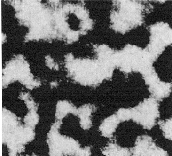
\includegraphics[width=0.3\columnwidth]{Figures/SlidesOWP200140903/MRF}
	%\caption{\label{fig:MRF} Synthetic image by (MRF) modeling  \cite{MRFTM}. }
 	%\end{figure}
	%
%By the use of approximations of \emph{Cliqués} we can describe joint probability models by considering a markovian property. For example, if we define $b_{u,v} = x_{i}$ with $i \in [N]$ and $ (u,v) \in [M] x [M]$ as a mapping transform (from our original stochastic field space without specific spatial order to a sorted \emph{2-D} space) and assuming a \emph{Cliqué} with only vertical and horizontal dependence of unitary distance $\scriptstyle{(\mathcal{N}(b_{u,v}) = \lbrace b_{u-1,v}, b_{u,v-1}, b_{u+1,v}, b_{u,v+1} \rbrace )}$ we can reduce the joint probability of a specific spatial variable by only considering the interaction with the members of it \emph{Cliqué} (only four variables in the neighborhood of this example). A realistic characterization of the \emph{Cliqué} will provides better estimation for the joint entropy while a simplified version of the \emph{Cliqué} will offer more computationally affordable implementations.
%
%%$\mathds{P}_{X}(X) = = \prod_{(j,k) \in [N x N]}{\Psi(b_{j,k},\mathcal{N}(b_{j,k}))} $
%
%We want to explore in detail this kind of markovian models in the next stages of this thesis.
%
%%where $\Psi(b_{j,k},\mathcal{N}(b_{j,k}))$ 
%%Joint Entropy $\scriptstyle{\tilde{H}(\Psi_{j,k}) = \sum_{b_{j,k} \in \mathcal{A}}{\Psi_{j,k} \log( \Psi_{j,k} )} }$
%%on $N$: 
%%$H(X)  =  \displaystyle \sum_{l = 1}^{k}{\tilde{H}(\Psi_{i_lj_l})}$
%
%%In the case of resolvability capacity for \emph{MRFs} we want to study definitions based on \emph{Cliqués}:
%%	$
%%	C_k  =  \displaystyle \frac{\displaystyle \max_{f_k \in \mathbf{F}_k} \displaystyle \sum_{l = 1}^{k}{\tilde{H}(\Psi_{i_lj_l})} }{\displaystyle \sum_{l = 1}^{M^2}{\tilde{H}(\Psi_{i_lj_l})}}
%%	$
%
%
%
%\subsection{Recapitulation and interpretation of implemented \emph{OWP} rules}
%
%An optimal (from \emph{information theoretic} approach) sensor placement rule for select $K$ measurements rely on the maximization of the prior entropy $H(X_f)$ with $f \in F$. By chain rule for entropy:
%
%
%\begin{equation}\label{eq_def_chain_rule}
	%H(X_f) = H(X_{f(1)}) + H(X_{f(2)}|X_{f(1)}) + \ldots + H(X_{f(K)}|X_{f(K-1)}, \ldots ,X_{f(1)} , )
%\end{equation}
%
%In preliminary formulation we considered the case of the initial $K$ measurements without previous sampled positions in the field. As iterative \emph{OWP} rules take measurements one by one or in groups we can rewrite the entropy isolating the positions previously measured. Thus, the expression of Eq. \eqref{eq_def_chain_rule} can be divided in two parts. Let $j$ be an index that accounts for the position of the $J$ variables that have been previously measured by a rule $\widetilde{f}$, before the current optimization process $f$ of $L = |f|$ new sampling positions is applied. Then,
%
%
%\begin{multline}\label{eq_def_chain_rule}
%H(X_f)  =  \sum_{j=1}^{J} H(X_{\widetilde{f}{(j)}} | X_{\widetilde{f}{(j-1)}},\ldots,X_{\widetilde{f}{(1)}}) + \\
           %\sum_{l = 1}^{L}H(X_{f(l)} | X_{f(l-1)},\ldots,X_{f(1)},   X_{\widetilde{f}{(J)}},X_{\widetilde{f}{(J-1)}},\ldots,X_{\widetilde{f}{(1)}} )
%\end{multline}
%
%The first sum is equal to zero, because it represent the uncertainty of a set of variables that are known already by the initial $J$ measurements. In addition, in the second sum we can recognizes two kind of conditioning variables as exposed in the definition Eq. \eqref{eq_def_conditionals}:
%
%\begin{equation}\label{eq_def_conditionals}
%X_{S_{l}} = \{  X_{f(l-1)},X_{f(l-2)},\ldots,X_f(1),   X_{\widetilde{f}{(J)}}, X_{\widetilde{f}{(J-1)}},\ldots,X_{\widetilde{f}{(1)}}  \}
%\end{equation}
%
%
%While variables indexed from rule $\widetilde{f}$ from $1, \ldots , J$ are previous sampling positions and the specific realization for each variable could be accessible by the measurement process, the variables indexed by the rule $f$ from $1, \ldots, L$ are the target of the current \emph{OWP} rule.
%
%For simplicity we can use a sorted combination $\widehat{f}$ of the rules $\widetilde{f}$ and $f$ with indexes from $1, \ldots, K$. Indexes from $1, \ldots, J$ account the positions obtained from the rule $\widetilde{f}$ and the indexes from $J+1, \ldots, K$ accounts the positions obtained from the rule $f$.
%
%\begin{equation}\label{eq_def_conditionals_joint}
%X_{S_{k}} = \{ X_{\widehat{f}(1)}, \ldots, X_{\widehat{f}(J)} , X_{\widehat{f}(J+1)}, \ldots, X_{\widehat{f}(K)} \}
%\end{equation}
%
%Now, by the entropy chain rule we have rewritten the initial method, as the sum of marginal entropy of each wanted sensor position and its conditionals. This representation keeps the problem from original formulation: As we are doing an optimization over a space of size ${L \choose [N] - J} $ the solution to this problem can be found by applying an algorithm of combinatorial complexity which is unfeasible or at least highly computationally intensive for fields with thousands or more variables. Instead, we propose to analyze each element separately in an iterative algorithm. 
%
%\begin{equation}\label{eq_numerical_OWP_4}
%X_f(i)^* = \argmax_{X_{ i } \in X} H(X_{ i }|X_{S_{i}})
%\end{equation}
%
%\begin{equation}\label{eq_def_entropy_cond}
%H(X_{ i }|X_{S_i}) = \sum_{x_{S_i} \in A^{|S_{i}|}} P(X_{S_i}) H(X_{ i } | X_{S_i} = x_{S_i})
%\end{equation}
%
%where $x_{S_i}$ denotes the set of values that $X_{S_i}$ takes in a particular realization. There is still a problem with the estimation of joint distribution for the variables we are optimizing on. To solve this problem, we can assume that $P(X_{S_i})$ follows a degenerated distribution after $X_{S_i}$ was measured with the realization $x^{0}_{S_i}$. This assumption allows us to rewrite Eq. \eqref{eq_def_entropy_cond} to:
%
%\begin{equation}\label{eq_def_entropy_cond}
%H(X_{ i }|X_{S_i}) =  H(X_{ i } | X_{S_i} = x^{0}_{S_i})
%\end{equation}
%
%This new equation reduce the number of degrees of freedom in the joint distribution. Therefore, we only need to estimate the probabilities of $X_{ i }$ in the alphabet $A$ conditioned to the specific $x^{0}_{S_i}$ realization. This conditional entropy can be easily estimated using pattern search tools or \emph{MPS} techniques for the case of \emph{2-D} channelized structures studied in this thesis.






















































































































































\section{Adaptive Sequential Empirical Maximum Entropy Sampling (\emph{AdSEMES}) using Previous Sensed Data}
\label{sec_Meth_Marginal}

The proposed \emph{OWP} formulations, from Eq. \eqref{eq:Meth_Theo_OWP_minH} and Eq. \eqref{eq:Meth_Iter_OWP_Itk}, are based on the knowledge of the statistics for the random regionalized variables. In practice, this theoretical model is not available and we need to find the way to estimate this model from empirical data. Sources of empirical statistics are reference images provided by experts, historical information or imposed models. From the iterative solution in Eq. \eqref{eq:Meth_Iter_OWP_Itk}, we formalize an appropriate framework to integrate these empirical sources. %In this work the use of training images and geostatistical simulation tools is proposed as a source for estimating the joint and conditional distributions of $X$. 

First, an optimal (from \emph{information theoretic} approach) sensor placement rule for select $K$ measurements is based on the maximization of the prior entropy $H(X_f)$ with $f \in F$. Using the chain rule of the entropy we hve that:


\begin{equation}\label{eq:Meth_Pract_OWP_ChainRuleH_1}
	H(X_f) = H(X_{f(1)}) + H(X_{f(2)}|X_{f(1)}) + \ldots + H(X_{f(K)}|X_{f(K-1)}, \ldots ,X_{f(1)} , )
\end{equation}

In the original formulation in section \ref{sec_Meth_fOSP}, we considered the case of the initial $K$ measurements without previous sampled positions in the field. As the iterative \emph{OWP} principle takes measurements in groups we can rewrite the entropy isolating the positions previously measured. Thus, Eq. \eqref{eq:Meth_Pract_OWP_ChainRuleH_1} can be divided in two parts. Let $j$ be an index that accounts for the position of the $J$ variables that have been previously measured by a rule $\widetilde{f}$, and $m$ the index for the current optimization process $f$ of $M = |f|$. Then,  %new sampling positions is applied. Then,


%\begin{multline}\label{eq_def_chain_rule}
%H(X_f)  =  \sum_{j=1}^{J} H(X_{\widetilde{f}{(j)}} | X_{\widetilde{f}{(j-1)}},\ldots,X_{\widetilde{f}{(1)}}) + \\
%           \sum_{l = 1}^{M}H(X_{f(l)} | X_{f(l-1)},\ldots,X_{f(1)},   X_{\widetilde{f}{(J)}},X_{\widetilde{f}{(J-1)}},\ldots,X_{\widetilde{f}{(1)}} ) .
%\end{multline}
\begin{align}\label{eq:Meth_Pract_OWP_ChainRuleH_2}
H(X_f) = & \sum_{j=1}^{J} H(X_{\widetilde{f}{(j)}} | X_{\widetilde{f}{(j-1)}},\ldots,X_{\widetilde{f}{(1)}}) + \nonumber \\
         & \sum_{m = 1}^{M}H(X_{f(m)} | X_{f(m-1)},\ldots,X_{f(1)},   X_{\widetilde{f}{(J)}},X_{\widetilde{f}{(J-1)}},\ldots,X_{\widetilde{f}{(1)}} ) .
\end{align}



The first sum is equal to zero, because each component $H(X_{\widetilde{f}{(j)}} = x_{\widetilde{f}{(j)}} | X_{\widetilde{f}{(j-1)}} = x_{\widetilde{f}{(j-1)}},\ldots,X_{\widetilde{f}{(1)}}) = x_{\widetilde{f}{(1)}}$ is equal to zero (the entropy of a degenerated variable is zero). In addition, in the second sum we can recognizes two kind of conditioning variables as exposed in the next definition:

\begin{equation}\label{eq:Meth_Pract_OWP_Xs}
X_{S_{m}} = \{  X_{f(m-1)},X_{f(m-2)},\ldots,X_{f(1)},   X_{\widetilde{f}{(J)}}, X_{\widetilde{f}{(J-1)}},\ldots,X_{\widetilde{f}{(1)}}  \} .
\end{equation}


While variables indexed from rule $\widetilde{f}$ from $1, \ldots , J$ are previous sampled positions and the specific realization for each variable could be accessible by the measurement process, the variables indexed by the rule $f$ from $1, \ldots, M$ are the target of the current \emph{OWP} rule.

For simplicity, we can use a sorted combination $\widehat{f}$, of the rules $\widetilde{f}$ and $f$ with indexes from $1, \ldots, K$. Indexes from $1, \ldots, J$ account the positions obtained from the rule $\widetilde{f}$ and the indexes from $J+1, \ldots, K$ accounts the positions obtained from the rule $f$. The we can define the subset of conditioning variables:

\begin{equation}\label{eq:Meth_Pract_OWP_XsJoint}
X_{S_{K}} = \{ X_{\widehat{f}(1)}, \ldots, X_{\widehat{f}(J)} , X_{\widehat{f}(J+1)}, \ldots, X_{\widehat{f}(K)} \} .
\end{equation}

%Now, by the entropy chain rule we have rewritten the initial method, as the sum of marginal entropy of each wanted sensor position and its conditionals. This representation 
%The maximization of target function from \eqref{eq_def_chain_rule} keeps the issue from original formulation: As we are doing an optimization over a space of size
To choose ${N - J \choose M} $ positions by the optimal rule $\widehat{f}$ still requiring an algorithm of combinatorial complexity which is unfeasible or at least highly computationally intensive for fields with thousands or more variables. Instead, we propose to analyze each element separately in an iterative algorithm. 

\begin{equation}\label{eq:Meth_Pract_OWP_maxH}
\widehat{i}^* = \argmax\limits_{\substack{i\in [N] \\ i \notin S_{i}}} H(X_{i}|X_{S_{i}}) ,
\end{equation}
with: 
\begin{equation}\label{eq:Meth_Pract_OWP_HCondXs}
H(X_{i}|X_{S_i}) = \sum_{x_{S_i} \in A^{|S_{i}|}} P(X_{S_i}) H(X_{i} | X_{S_i} = x_{S_i}) .
\end{equation}

Here, $x_{S_i}$ denotes the set of values that $X_{S_i}$ takes in a particular realization. %There is still a problem with the estimation of joint distribution for the variables we are optimizing on. 
In our iterative approach, we can assume that $P(X_{S_i})$ follows a degenerated distribution after $X_{S_i} = x^{0}_{S_i}$ was measured. This assumption allows us to rewrite Eq. \eqref{eq:Meth_Pract_OWP_HCondXs} to:

\begin{equation}\label{eq:Meth_Pract_OWP_HCondXsMeasured}
H(X_{i}|X_{S_i}) =  H(X_{i} | X_{S_i} = x^{0}_{S_i}) .
\end{equation}

The Eq. \eqref{eq:Meth_Pract_OWP_HCondXsMeasured} reduces the number of degrees of freedom in the joint distribution. Therefore, we only need to estimate the probabilities of $X_{i}$ in the alphabet $A$ conditioned to the specific $x^{0}_{S_i}$ realization. This conditional entropy can be easily estimated using pattern search tools or \emph{MPS} techniques for the case of \emph{2-D} channelized structures studied in this work.





















\subsection{Stopping Rule via $\mathcal{C}_{K}$ Evolution}
\label{sec_Meth_StopRules}

A key topic related with adaptive sampling strategies is to determine a robust method for stopping the sampling process. The objective is to set a limit on the number of samples.For this we propose a stopping critaria based on the resolvability capacity of the field. 

In particular, we propose the use of the monotonically increasing sequence $\mathcal{\tilde{C}}_{K}$ in the iterative sampling scheme. Using the Eq. \eqref{eq:Meth_Iter_OWP_Ck}, the change in the resolvability capacity factor, after taking an additional measure, is given by:

\begin{align}\label{eq:StopRule_Iter_DeltaCk}
	\Delta \mathcal{\tilde{C}}_{K} & = \mathcal{\tilde{C}}_{K} - \mathcal{\tilde{C}}_{K-1} \\
																 & = \frac{I(\tilde{f}^{*}_{K})- I(\tilde{f}^{*}_{K-1})}{H(X)} \nonumber \\																 & \propto H(X_{ i^{*}_{K} }|X_{ i^{*}_{1} },\ldots,X_{ i^{*}_{k-1} }) \nonumber
\end{align}


The use of this proportional version is supported by the fact that the joint entropy for the field $X$ is the same throughout the sensing process, but inaccessible in practical applications. Therefore, we consider $H(X)$ as a scale factor and, consequently, we omit this factor as shown in Eq. \eqref{eq:StopRule_Iter_DeltaCk}. For the iterative approach, from Eq. \eqref{eq:Meth_Iter_OWP_Itk}, $\mathcal{\tilde{C}}_{K}$ is a monotonically decreasing sequence as $K \rightarrow N$. In particular, when  $\mathcal{\tilde{C}}_{k_{limit}} = 0$ for a $k_{limit} \in {1, \ldots, K}$ the remaining non measured $N - k_{limit}$ random variables are deterministically determined by the variables indexed by the rule $\tilde{f}^{*}_{k_{limit}}$. Then, no more information will be obtained for the random field by additional measures and the sensing process must be truncated.

% From monotonically increasing nature of $\mathcal{\tilde{C}}_{K}$,  $\Delta \mathcal{\tilde{C}}_{K}$ is a monotonically decreasing sequence as $K \rightarrow N$. Finally, when $\Delta \mathcal{\tilde{C}}_{k} = 0$ after $k$ sequential measures, no more information will be obtained from the field by additional measures and the sensing process must be truncated. 

























%\subsection{Estimation of the Stochastic Field Model from empirical statistics}
%\label{sec_Meth_Estimation}



%We will explore an \emph{OWP} acquisition system where the pixel entropy estimation is based on MPS simulations analysis as presented in fig. \ref{fig:owpmps}.
%
%\begin{figure}[ht!]
    %\centering
    %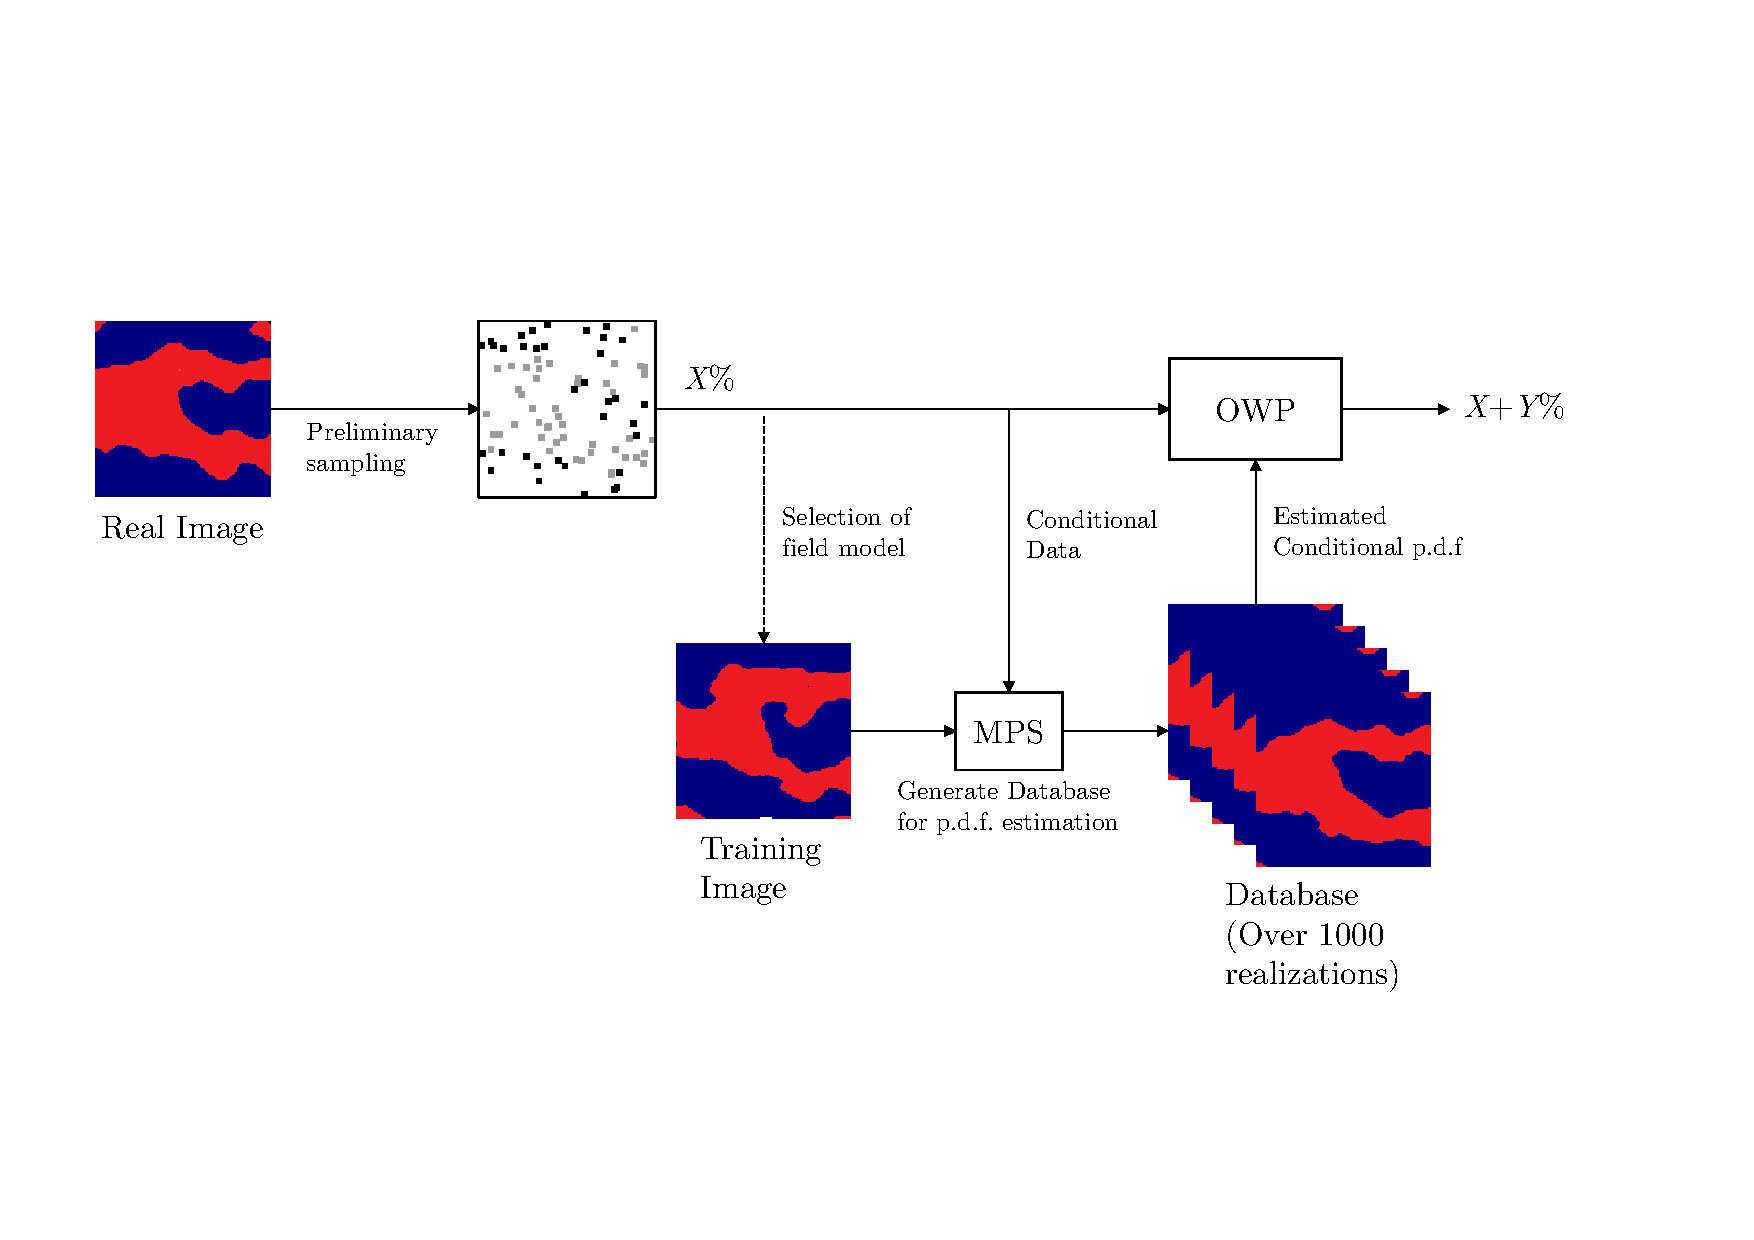
\includegraphics[width=1\columnwidth]{Figures/IDSDAY2015/OWP_MPS}
	%\caption{\label{fig:owpmps} OWP-MPS acquisition scheme}
%\end{figure}
%
%In sequential sensing is possible to update the probabilities after a new observation is available. This MPS enhanced scheme is shown in fig. \ref{fig:owpmpsenhc}.
 %
%\begin{figure}[ht!]
    %\centering
    %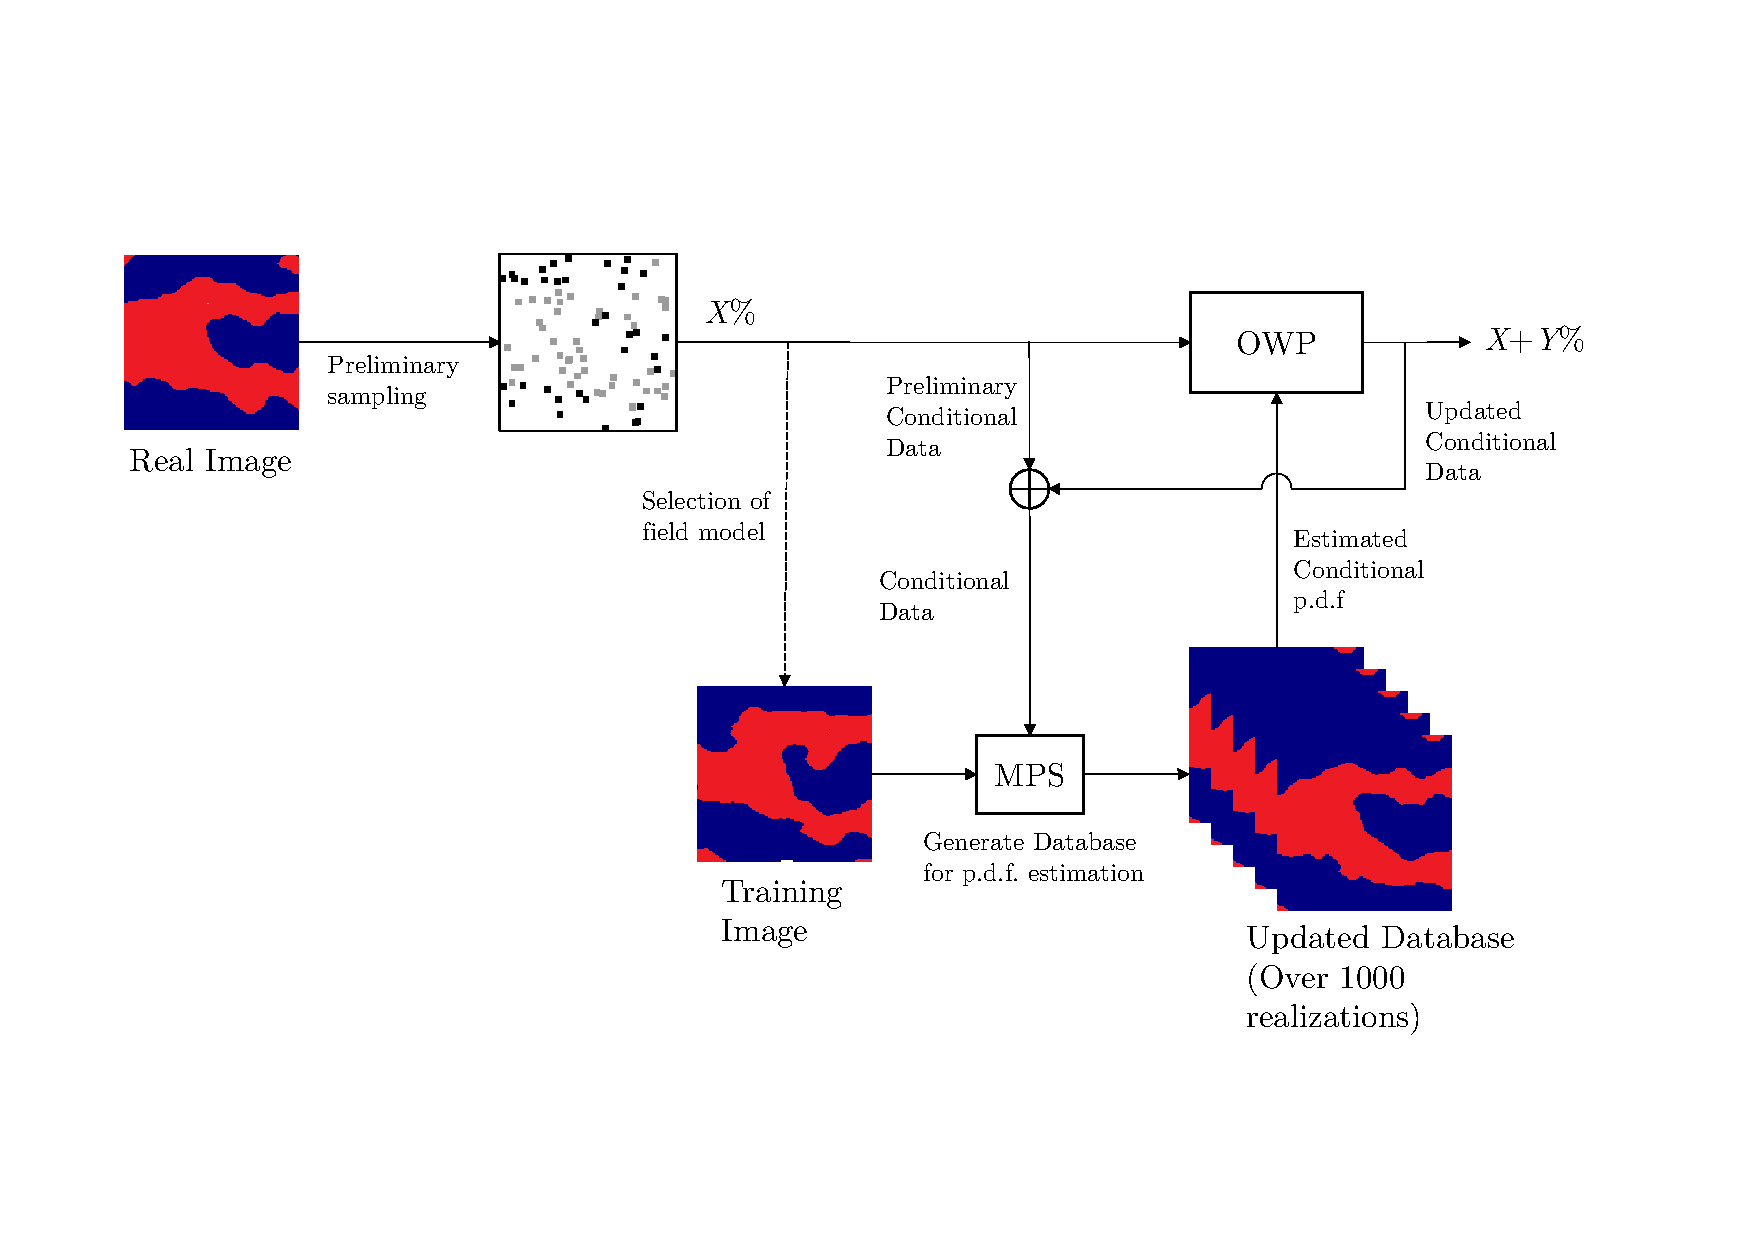
\includegraphics[width=1\columnwidth]{Figures/IDSDAY2015/OWP_MPS_ENHACED}
	%\caption{\label{fig:owpmpsenhc}OWP-MPS Enhanced acquisition scheme}
%\end{figure}
%
%Finally, we propose to bypass the use of \emph{MPS} and use the training image instead by pattern search based probabilities estimation (fig. \ref{fig:owptips}).
%
%\begin{figure}[ht!]
    %\centering
    %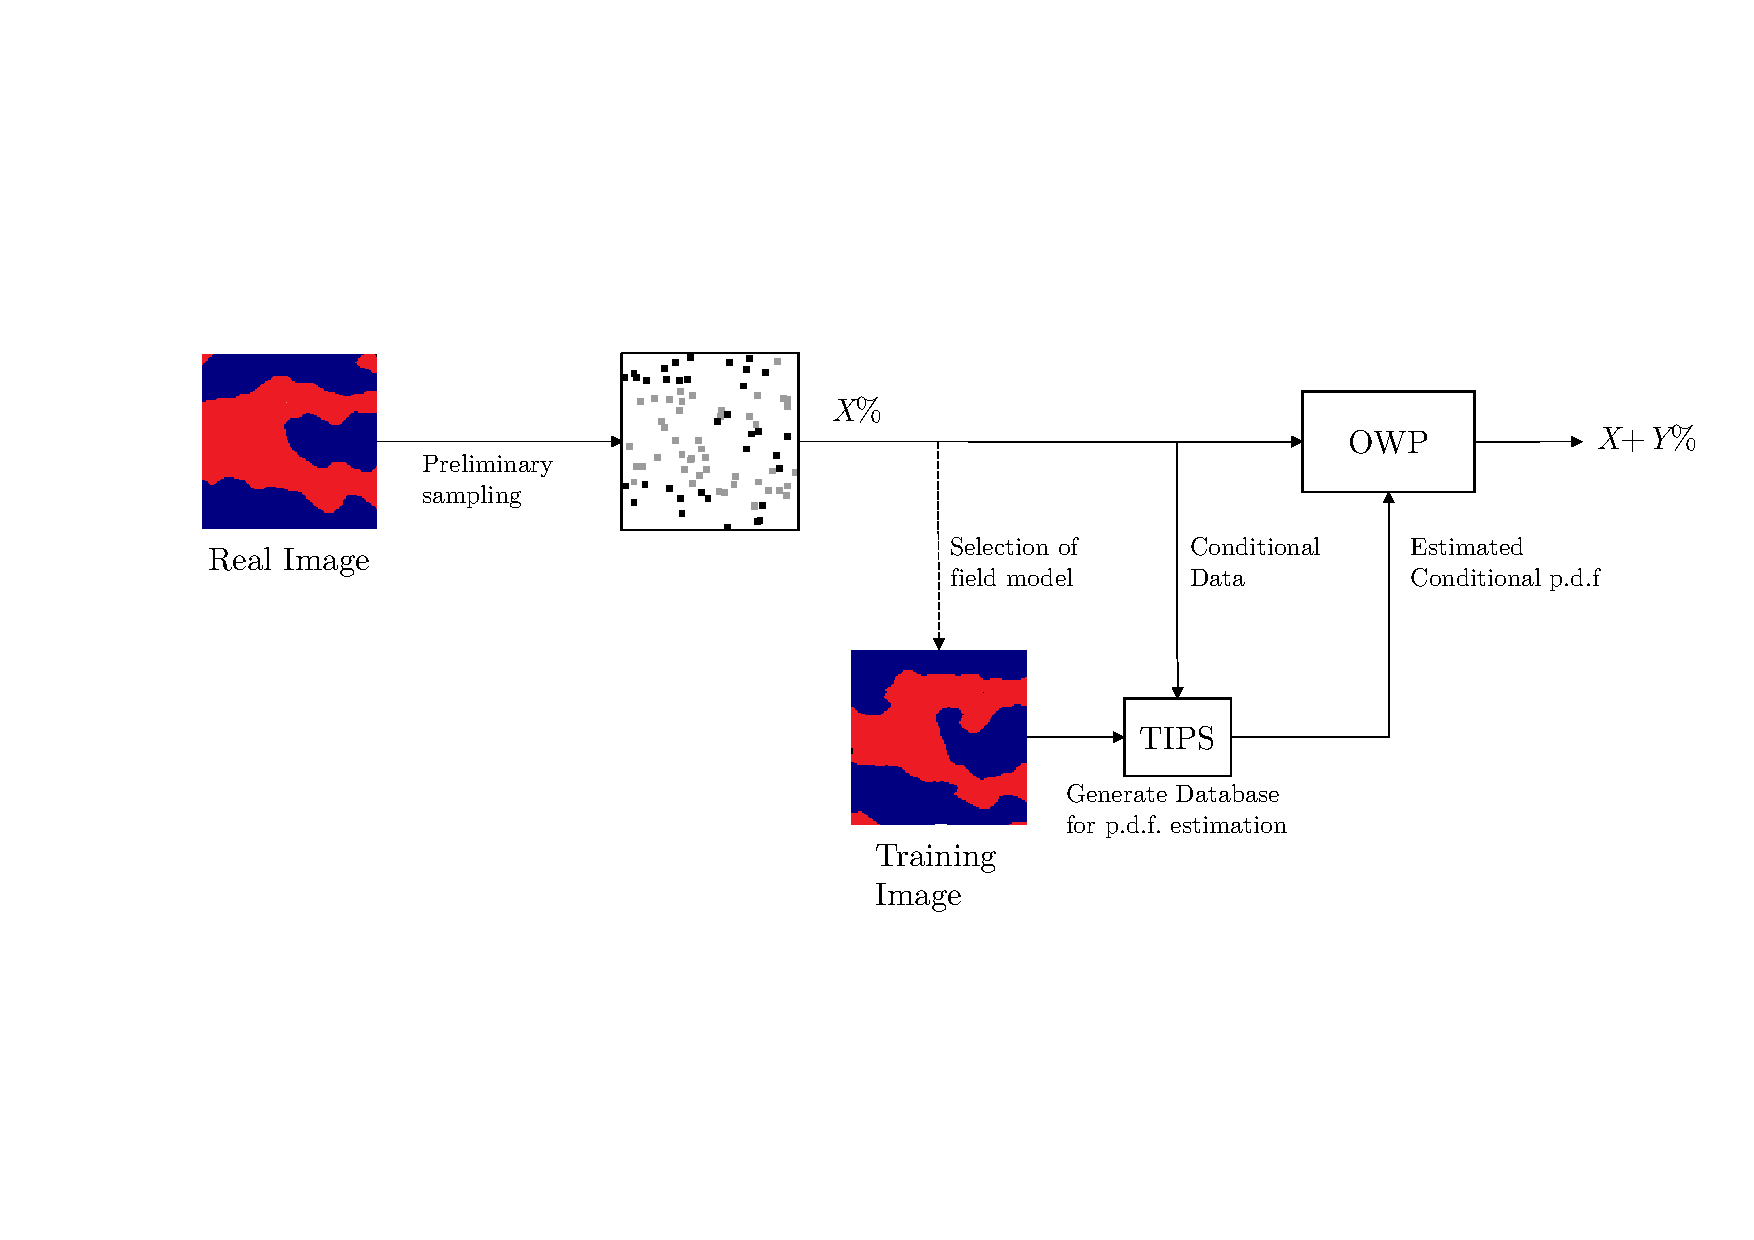
\includegraphics[width=1\columnwidth]{Figures/IDSDAY2015/OWP_TIPS}
	%\caption{\label{fig:owptips} TIPS acquisition scheme}
%\end{figure}
%





























































































%%%%%%%%%%%%%%%%%%%%%%%%%%%%%%%%%%%%%%%%%%%%%%%%%%%%%%%%%%%%%%%%%%%%%%%%%%%%%%%%%%%
%%%%%%%%%%%%%%%%%%%%%%%%%%%%%%%%%%%%%%%%%%%%%%%%%%%%%%%%%%%%%%%%%%%%%%%%%%%%%%%%%%%
%%%%%%%%%%%%%%%%%%%%%%%%%%%%%%%%%%%%%%%%%%%%%%%%%%%%%%%%%%%%%%%%%%%%%%%%%%%%%%%%%%%
%%%%%%%%%%%%%%%%%%%%%%%%%%%%%%%%%%%%%%%%%%%%%%%%%%%%%%%%%%%%%%%%%%%%%%%%%%%%%%%%%%%
%%%%%%%%%%%%%%%%%%%%%%%%%%%%%%%%%%%%%%%%%%%%%%%%%%%%%%%%%%%%%%%%%%%%%%%%%%%%%%%%%%%
%%%%%%%%%%%%%%%%%%%%%%%%%%%%%%%%%%%%%%%%%%%%%%%%%%%%%%%%%%%%%%%%%%%%%%%%%%%%%%%%%%%
%%%%%%%%%%%%%%%%%%%%%%%%%%%%%%%%%%%%%%%%%%%%%%%%%%%%%%%%%%%%%%%%%%%%%%%%%%%%%%%%%%%
\section{Experimental Results}

Based on our formalization of the near optimal measurements location in Eq. \eqref{eq:Meth_Pract_OWP_HCondXsMeasured}, we implemented an iterative \emph{OWP} solution and provided a comparison between \emph{OWP} and structured/randomized sampling schemes. Our scheme consider the stages exposed in the fig. \ref{fig:SytemOWP_MPS}.

\begin{figure}[h!]
    \centering
    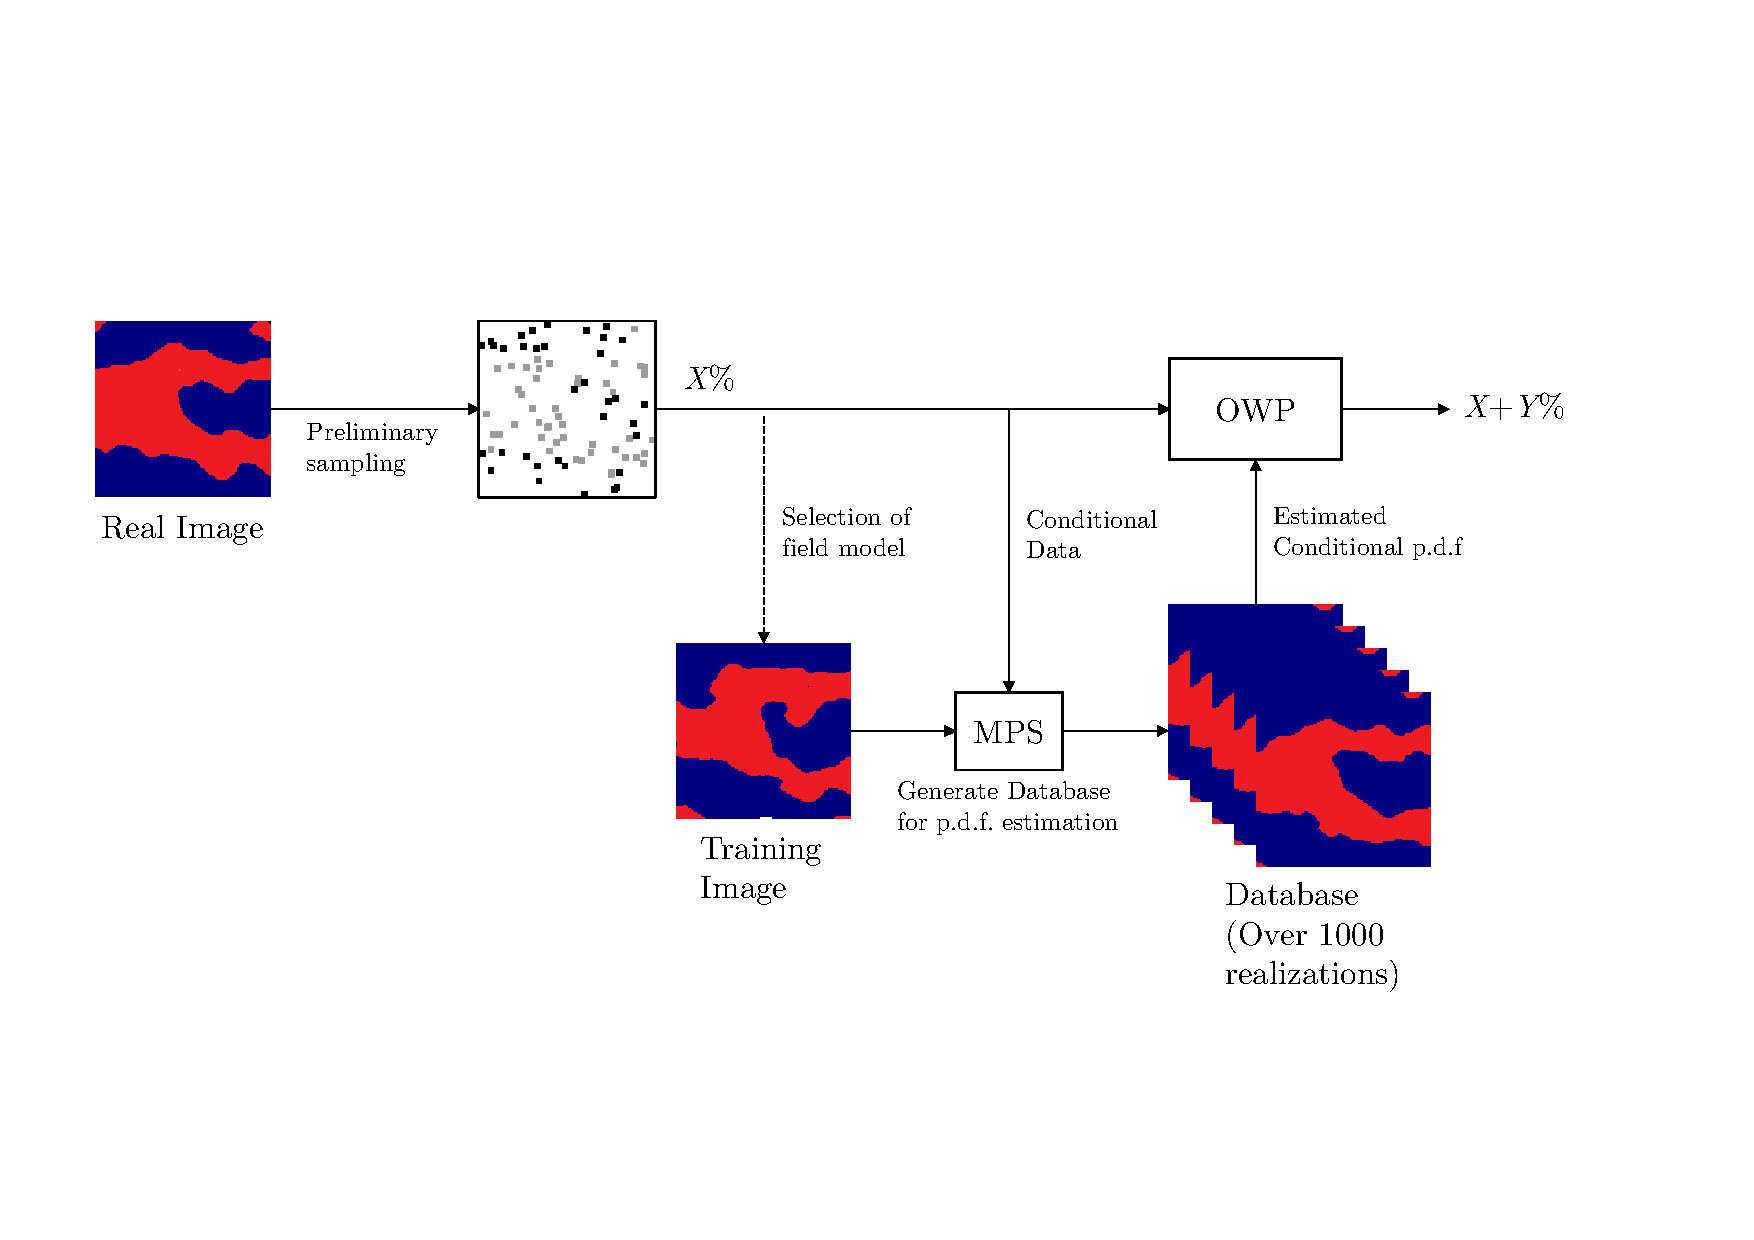
\includegraphics[width=0.85\columnwidth]{Figures/IDSDAY2015/OWP_MPS.pdf}
	\caption{\label{fig:SytemOWP_MPS} Proposed Inference system.}
 \end{figure}


\subsection{Data Base}

The Database used in our preliminary experiments considered the next constrains: \

	\tikzset{blocknode/.style={inner sep=0,text width=1\textwidth,below right}}

	\begin{tikzpicture}
	\node[blocknode] {\begin{itemize}\item Nature 	\item Dimensionality \item Variable \item Dimensions \item Type \item Source \end{itemize}};
	\node[blocknode] at (0.5\textwidth,0) {\begin{itemize}\item[$\rightarrow$] Discrete random field \item[$\rightarrow$] \emph{2-D} \item[$\rightarrow$] Permeability \item[$\rightarrow$] $200 \times 200$ px	\item[$\rightarrow$] Bi-categorical \item[$\rightarrow$] synthetic realizations \end{itemize}};
	\end{tikzpicture}


\subsection{Experiments}

We considered the next approach to evaluate the sampling design using the proposed database: \

\begin{itemize}
\item Iterative \emph{OWP} version.
\item Combined sampling scheme (uniform sampling (structured) + \emph{OWP} ) with an initial presampled positions.
\item $200$ \emph{MPS} realizations for statistics estimation.
\end{itemize}

For example, from database we select the next image as the realization image describing the actual channels structure in the subsurface:


\begin{figure}[ht!]
    \centering
    
\includegraphics[width=0.2\columnwidth]{Figures/SlidesOWP200140903/r_209.png}
	\caption{\label{fig:groundtruth} Realization Image. }
 \end{figure}

First, we used an initial uniform structured sampling\footnotemark \ and then we applied \emph{OWP} approach. We overall sampling consisted of the $2\%$ samples from the available positions in the field (realization image). Our modified \emph{OWP} sampling take into account the next heuristics rules: \footnotetext{Needed to the right representation of bad conditioned zones, required for the use of \emph{MPS} as a posterior inference system}

\begin{itemize}
\item \small Selection of closest conditionals for \textbf{each available position for sampling} ($9$ nearest point in preliminary heuristic implementation).
\item \small Estimation of conditional probabilities by histograms for \emph{MPS} simluations.
\item \small Estimation of entropy maps.
\item \small Selection of maximal entropy candidates and heuristic corrections.
\end{itemize}


\subsection{Preliminary Experimental Results}\label{sec_exp_OWP}

Our experimental setting considered binary images that represent permeability fields. The experiments consisted on the comparison between an equally spaced sensing system and a mixed approach that includes equally spaced measurements and measurements given by the iterative algorithms proposed in Eq. \eqref{eq:Meth_Pract_OWP_HCondXsMeasured}. The objective of this comparison is to contrast the effect that sensing design produces on the \emph{posteriori} entropy map of the field $X$. For that, simulations \emph{MPS} tool is also evaluated (by SNESIM algorithm)\cite{huang_2013_a}. The \emph{MPS} technique utilizes a training image, provided by expert knowledge, to perform simulated images that conserve the patterns present in the reference image. In addition, the \emph{MPS} method can be conditioned by measured data.

The first approach consisted on an equally spaced samples of the actual realization field. The second apporach is described in Fig. \ref{fig:SytemOWP_MPS}. It required a small portion of preliminary data given by the first method and the other portion sequentially obtained by the application of Eq.\eqref{eq:Meth_Pract_OWP_HCondXsMeasured}. Conditional probability \emph{PDF}s will be estimated using the representative database generated from the simulation algorithm \cite{huang_2013_a,Ortiz_2004_a}, which uses \emph{MPS}. Using a frequentist approach, the probability that current pixel takes a specific value is estimated from the simulated data, for each value of the alphabet $\mathcal{A}$ (in this case, $|\mathcal{A}|=2$). Doing this operation for each position within $f^c$, we obtained an estimation of:

\begin{equation}\label{eq_sec_exp_1}
\mathds{P}(X_{ \{i \} } | X_{f}), \quad \forall i \in f^c
\end{equation}

Equipped with this empirical estimation of the posterior probabilities, we computed the conditional entropy, required to apply the \emph{OWP} algorithm proposed in Eq.\eqref{eq:Meth_Pract_OWP_HCondXsMeasured}. The analysis of the results relies on the behavior that the \emph{posteriori} entropy as can be seen in Fig. \ref{fig:experiments}. In this case, white pixels represents a high uncertainty zones, while black pixels means a strong knowledge of the value that the unobserved pixel is taking. As expected, for the scheme in which \emph{OWP} is included, the uncertainty is significantly reduced with respect to the other method. Both methods use the same amount of measurements ($2\%$ of all $N = 200 \cdot 200$ pixels), but in the one presented in this proposal, we used $X\%$ uniformly sampled and $Y\%$ by our \emph{OWP} method, where $X+Y =2\%$.

\begin{figure}[!h]
\centerline{
	\begin{subfigure}[b]{0.2\textwidth}
				\setlength{\fboxsep}{0.2pt}%
				\setlength{\fboxrule}{0.2pt}%
                \fbox{
\includegraphics[width=\textwidth]{Figures/ICASS2015/muestreo_equispaciado_parcial}}
              	  \label{fig:muestreo_1}
	\end{subfigure}	
	\begin{subfigure}[b]{0.2\textwidth}
				\setlength{\fboxsep}{0.2pt}%
				\setlength{\fboxrule}{0.2pt}%
                \fbox{
\includegraphics[width=\textwidth]{Figures/ICASS2015/muestreo_equispaciado_completo}}
                \label{fig:muestreo_2}
	\end{subfigure}
	\begin{subfigure}[b]{0.2\textwidth}
				\setlength{\fboxsep}{0.2pt}%
				\setlength{\fboxrule}{0.2pt}%
								\fbox{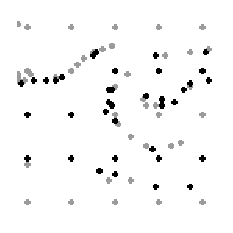
\includegraphics[width=\textwidth]{Figures/ICASS2015/muestreo_equispaciado_OWP}}
                \label{fig:muestreo_3}
	\end{subfigure}
}
\vspace{-0.3cm}
\centerline{
	\begin{subfigure}[b]{0.2\textwidth}
                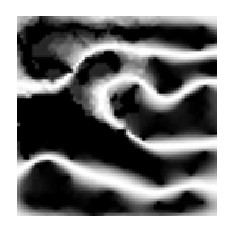
\includegraphics[width=\textwidth]{Figures/ICASS2015/entropy_equispaciado_parcial}
                \label{fig:entropy_1}
	\end{subfigure}
	\begin{subfigure}[b]{0.2\textwidth}
                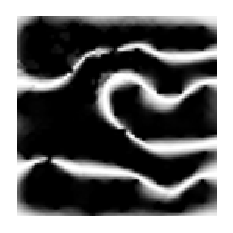
\includegraphics[width=\textwidth]{Figures/ICASS2015/entropy_equispaciado_completo}
                \label{fig:entropy_2}
	\end{subfigure}
	\begin{subfigure}[b]{0.2\textwidth}
                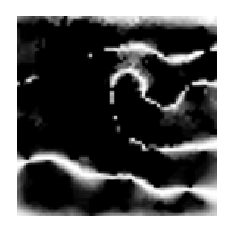
\includegraphics[width=\textwidth]{Figures/ICASS2015/entropy_equispaciado_OWP}
                \label{fig:entropy_3}
	\end{subfigure}
}
\caption{\label{fig:experiments} Preliminary experiment for adaptive sampling design.}
\scriptsize{Both measurement systems are shown with their \emph{posteriori} entropy map respectively. In the left column partial measurement process ($25$ uniformly sampled measurements) is shown previous to the \emph{OWP} application. In the middle one, equally spaced sampling method is presented for the $2 \%$ of samples. Finally, in the right column, the result after applying \emph{OWP} measurements is shown.}
\end{figure}

Next step was to generate simulations of the media using \emph{MPS} tool and using the samples provided by the various methods explained above. Using the samples acquired by different sampling schemes, we explored if there is a regime that combines equally spaced data sampling with data sampled through our method, that is near optimal from the point of view of entropy reduction, average reconstruction error, or variability of the \emph{MPS} simulations. Two metrics were proposed to measure performance: Signal-to-Noise ratio (SNR) between simulations and the reference image in order to analyze the quality of the realizations; and standard deviation of simulations, to measure the uncertainty introduced.

\begin{figure}[!h]
\centerline{
	\begin{subfigure}[b]{0.2\textwidth}
                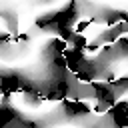
\includegraphics[width=\textwidth]{Figures/ICASS2015/std_00_equies_200_sim}
              	  \label{fig:std_1}
	\end{subfigure}	
	\begin{subfigure}[b]{0.2\textwidth}
                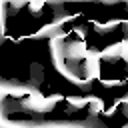
\includegraphics[width=\textwidth]{Figures/ICASS2015/std_06_equies_200_sim}
                \label{fig:std_2}
	\end{subfigure}
	\begin{subfigure}[b]{0.2\textwidth}
				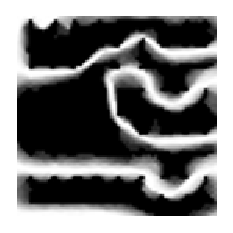
\includegraphics[width=\textwidth]{Figures/ICASS2015/std_10_equies_200_sim}
                \label{fig:std_3}
	\end{subfigure}
	}
\caption{\label{fig:std_ind} Standard deviation maps for different sampling schemes.}
\scriptsize{From left to right we have: full OWP, $60\%$ equally spaced sampling and $40\%$ OWP (optimal from SNR point of view) and a full equally spaced sampling scenario.}
\end{figure}

\begin{table}[!h]
\centering
\caption{\label{tab:metrics} Summary of performance for the \emph{OWP} experiment. }
$|\mathbf{\sigma}|$ corresponds to the total energy present in the standard deviation map. \\
 $<$SNR$>$ denotes mean \emph{S.N.R} between simulations and \emph{RI}. \\

  \begin{center}
  \begin{tabular}{ | c | c | c | c | c | c | c |}
  	\hline
  	Metric & $0\%$ & $20\%$ & $40\%$ & $60\%$ & $80\%$ & $100\%$\\
    \hline
    \tiny{$<$SNR$>$} & 13.9218 & 20.0376 & 23.2711 & 28.1413  & 22.9547 & 28.1044 \\
    $|\mathbf{\sigma}|$ & 18.2311 & 17.8426 & 13.0801 & 11.1337 & 10.3974 & 11.605 \\    
    \hline   
  \end{tabular}
  \end{center}
   
\end{table}

We performed $200$ simulations for each sampling scheme. As indicated before, we considered the scenario where $2\%$ of samples are available to do the reconstructions based on simulations. The mixed scheme considers $0 \%, 20 \%, 40 \%, 60 \%, 80 \%$ and $100 \%$ of equally spaced data, and the results are shown in Table \ref{tab:metrics}. The percentages shown in the first row make reference to the portion of equally spaced data used by the mixed method. From a $<$SNR$>$ point of view, the optimal case is obtained when combining $60\%$ of equally spaced data and $40\%$ acquired through OWP method (see Fig. \ref{fig:mean_error}). For the standard deviation case, optimum is placed in the range of the $80-20\%$ combination (see Fig. \ref{fig:std_ind}). These results indicated that both kind of data placement methods are complementary and that there exists a trade-off between characterization and uncertainty reduction. Provided results were coherent with the proposed algorithm nature that attempt to reduce global uncertainty on the overall process.

\begin{figure}[!t]
\centerline{
	\begin{subfigure}[b]{0.2\textwidth}
				
\includegraphics[width=\textwidth]{Figures/ICASS2015/imagen_referencia}
				\caption{}
                \label{fig:ref_image}
	\end{subfigure}
	\begin{subfigure}[b]{0.2\textwidth}
                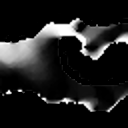
\includegraphics[width=\textwidth]{Figures/ICASS2015/mean_error_00}
                \caption{}
              	\label{fig:mean_error_0_equis}
	\end{subfigure}
	}
	%\vspace{-0.4cm}	
\centerline{
	\begin{subfigure}[b]{0.2\textwidth}
                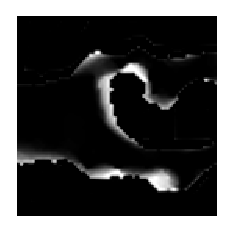
\includegraphics[width=\textwidth]{Figures/ICASS2015/mean_error_60}
                \caption{}
                \label{fig:mean_error_60_equis}
	\end{subfigure}
	\begin{subfigure}[b]{0.2\textwidth}
				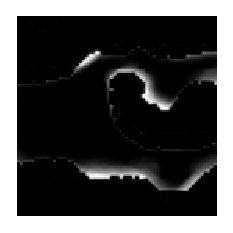
\includegraphics[width=\textwidth]{Figures/ICASS2015/mean_error_100}
				\caption{}
                \label{fig:mean_error_100_equis}
	\end{subfigure}	
	}
\caption{\label{fig:mean_error} Mean error for sampling schemes.}
\scriptsize{ a) Reference Image. b) Mean absolute error of full OWP scheme. c) Mean absolute error of $60\%$ equally spaced and $40\%$ OWP scheme. d) Mean absolute error of full equally spaced scheme.}
\end{figure}



%\subsection{Simulaciones}
%
%{Experimentos}
%\begin{figure}[H]
%\centering
%\centerline{
			%\begin{subfigure}[b]{0.33\textwidth}
				%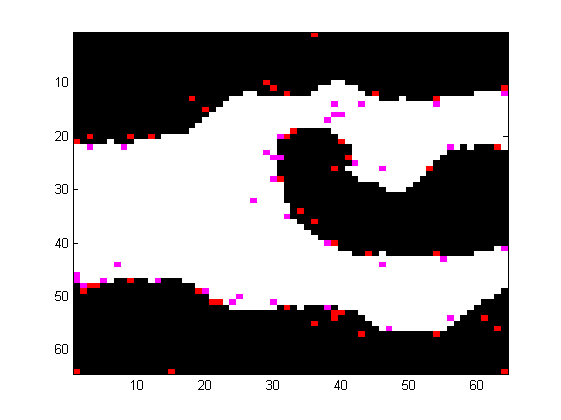
\includegraphics[width=\textwidth]{Figures/SlidesOWP200140903/muestreo_frac_aleat_0_percent_2}
				%\caption{0\% Eq. - 100\% OWP}
			%\end{subfigure}
			%\begin{subfigure}[b]{0.33\textwidth}
				%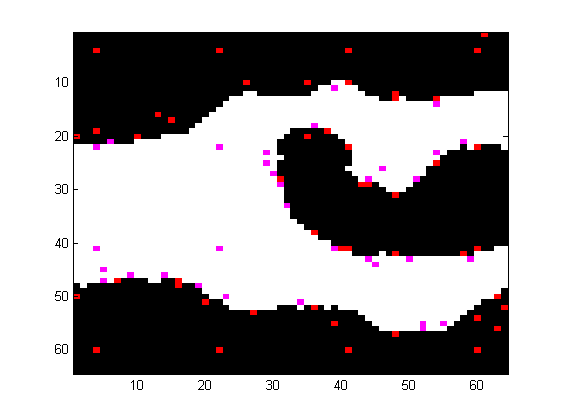
\includegraphics[width=\textwidth]{Figures/SlidesOWP200140903/muestreo_frac_aleat_02_percent_2}
				%\caption{20\% Eq. - 80\% OWP}
			%\end{subfigure}		
			%\begin{subfigure}[b]{0.33\textwidth}
				%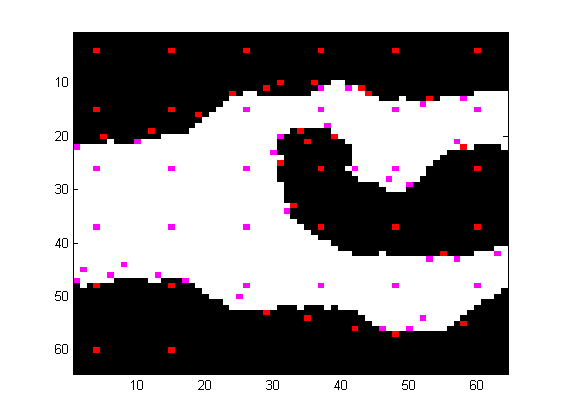
\includegraphics[width=\textwidth]{Figures/SlidesOWP200140903/muestreo_frac_aleat_04_percent_2}
				%\caption{40\% Eq. - 60\% OWP}
			%\end{subfigure}		
%}
%\centerline{
			%\begin{subfigure}[b]{0.33\textwidth}
				%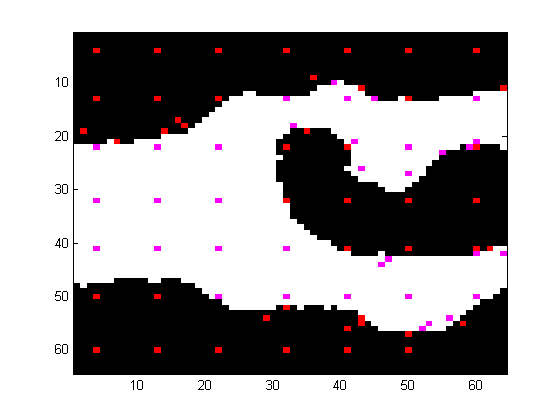
\includegraphics[width=\textwidth]{Figures/SlidesOWP200140903/muestreo_frac_aleat_06_percent_2}
				%\caption{60\% Eq. - 40\% OWP}
			%\end{subfigure}		
			%\begin{subfigure}[b]{0.33\textwidth}
				%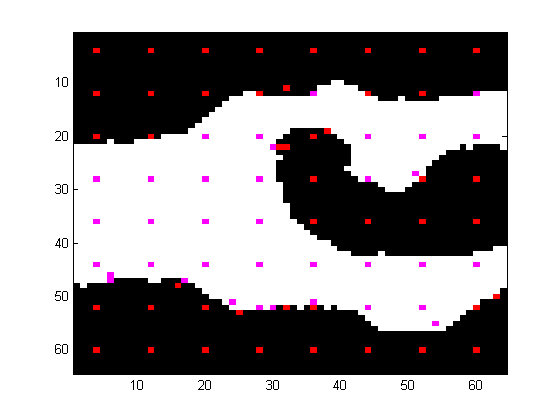
\includegraphics[width=\textwidth]{Figures/SlidesOWP200140903/muestreo_frac_aleat_08_percent_2}
				%\caption{80\% Eq. - 20\% OWP}
			%\end{subfigure}		
			%\begin{subfigure}[b]{0.33\textwidth}
				%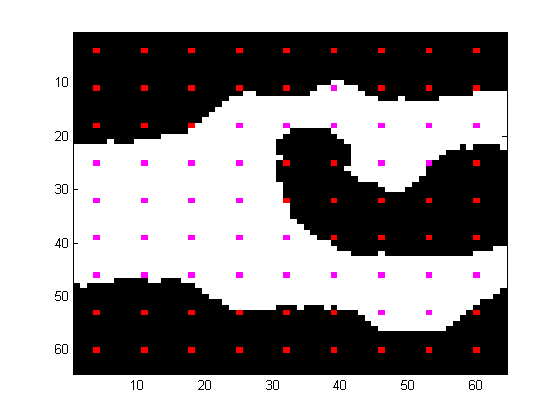
\includegraphics[width=\textwidth]{Figures/SlidesOWP200140903/muestreo_frac_aleat_10_percent_2}
				%\caption{100\% Eq. - 0\% OWP}
			%\end{subfigure}		
%}
%\caption[OWP más muestreo equiespaciado]{\label{fig:owpmuestreo}Muestreo para distintos porcentajes de muestreo equiespaciado.}
%\end{figure}
 %
%{Experimentos}
%\begin{figure}[H]
%\centering
%\centerline{
			%\begin{subfigure}[b]{0.33\textwidth}
				%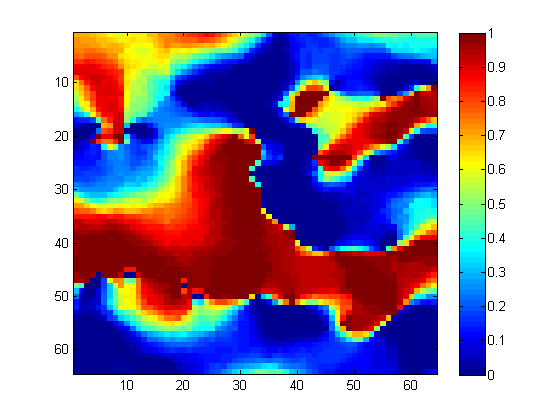
\includegraphics[width=\textwidth]{Figures/SlidesOWP200140903/mean_frac_aleat_0_percent_2}
				%\caption{0\% Eq. - 100\% OWP}
			%\end{subfigure}
			%\begin{subfigure}[b]{0.33\textwidth}
				%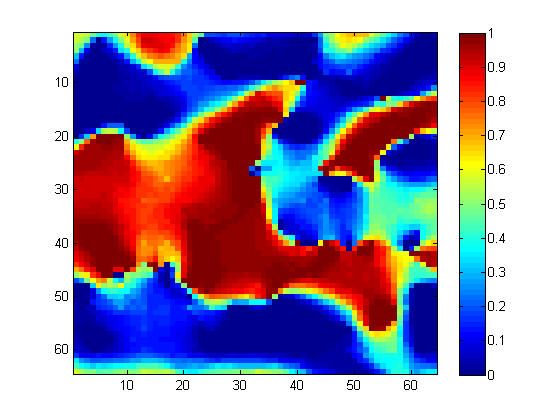
\includegraphics[width=\textwidth]{Figures/SlidesOWP200140903/mean_frac_aleat_02_percent_2}
				%\caption{20\% Eq. - 80\% OWP}
			%\end{subfigure}		
			%\begin{subfigure}[b]{0.33\textwidth}
				%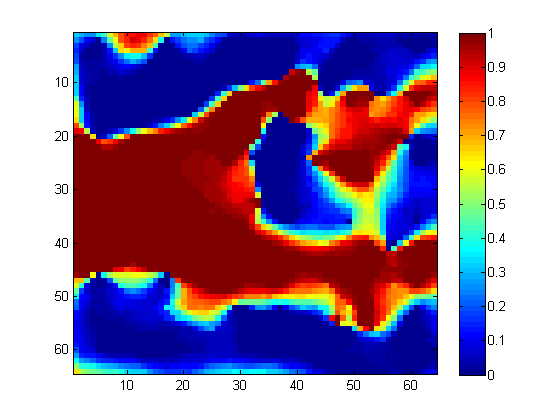
\includegraphics[width=\textwidth]{Figures/SlidesOWP200140903/mean_frac_aleat_04_percent_2}
				%\caption{40\% Eq. - 60\% OWP}
			%\end{subfigure}		
%}
%\centerline{
			%\begin{subfigure}[b]{0.33\textwidth}
				%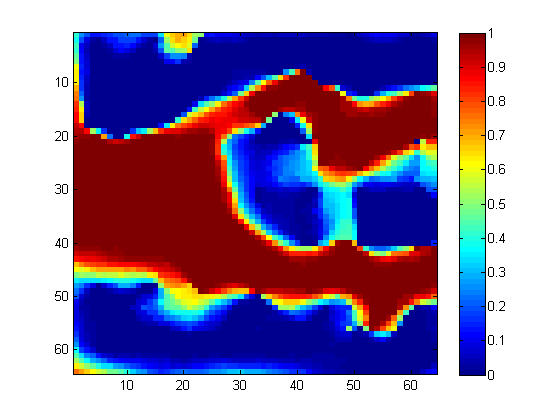
\includegraphics[width=\textwidth]{Figures/SlidesOWP200140903/mean_frac_aleat_06_percent_2}
				%\caption{60\% Eq. - 40\% OWP}
			%\end{subfigure}		
			%\begin{subfigure}[b]{0.33\textwidth}
				%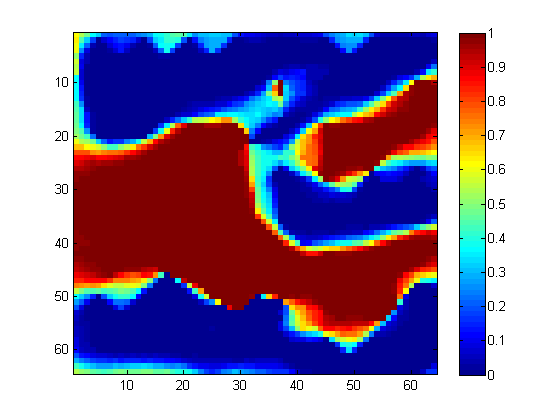
\includegraphics[width=\textwidth]{Figures/SlidesOWP200140903/mean_frac_aleat_08_percent_2}
				%\caption{80\% Eq. - 20\% OWP}
			%\end{subfigure}		
			%\begin{subfigure}[b]{0.33\textwidth}
				%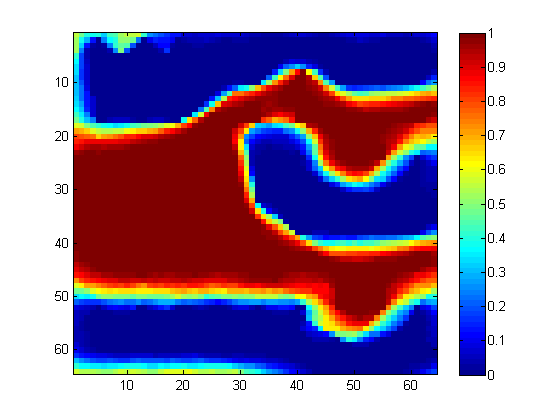
\includegraphics[width=\textwidth]{Figures/SlidesOWP200140903/mean_frac_aleat_10_percent_2}
				%\caption{100\% Eq. - 0\% OWP}
			%\end{subfigure}		
%}
%\caption[OWP más muestreo equiespaciado]{\label{fig:owppromedio} Imágenes Promedio de 200 simulaciones con MPS para distintos porcentajes de muestreo equiespaciado.}
%\end{figure}
%
%
 %
%{Experimentos}
%\begin{figure}[H]
%\centering
%\centerline{
			%\begin{subfigure}[b]{0.33\textwidth}
				%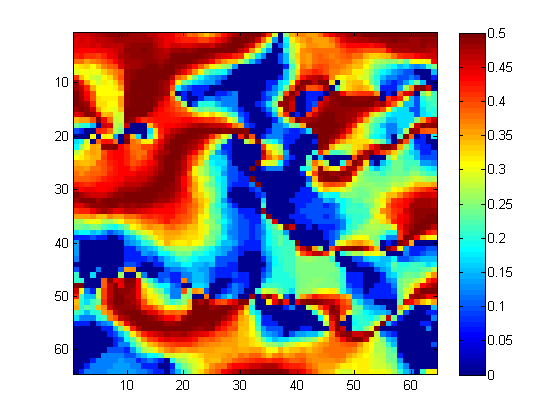
\includegraphics[width=\textwidth]{Figures/SlidesOWP200140903/std_frac_aleat_0_percent_2}
				%\caption{0\% Eq. - 100\% OWP}
			%\end{subfigure}
			%\begin{subfigure}[b]{0.33\textwidth}
				%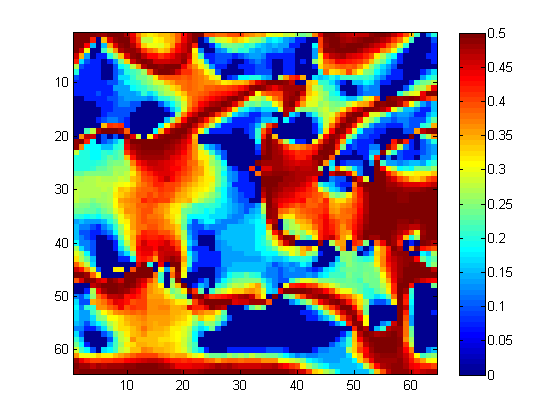
\includegraphics[width=\textwidth]{Figures/SlidesOWP200140903/std_frac_aleat_02_percent_2}
				%\caption{20\% Eq. - 80\% OWP}
			%\end{subfigure}		
			%\begin{subfigure}[b]{0.33\textwidth}
				%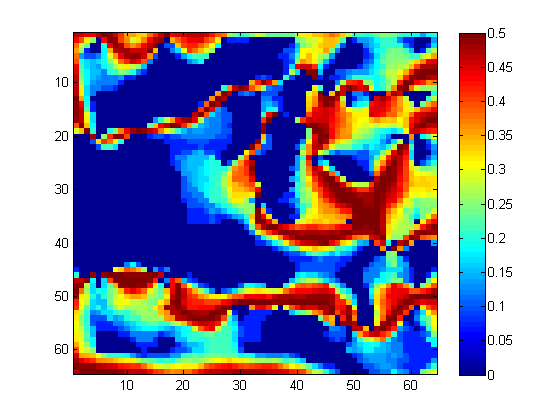
\includegraphics[width=\textwidth]{Figures/SlidesOWP200140903/std_frac_aleat_04_percent_2}
				%\caption{40\% Eq. - 60\% OWP}
			%\end{subfigure}		
%}
%\centerline{
			%\begin{subfigure}[b]{0.33\textwidth}
				%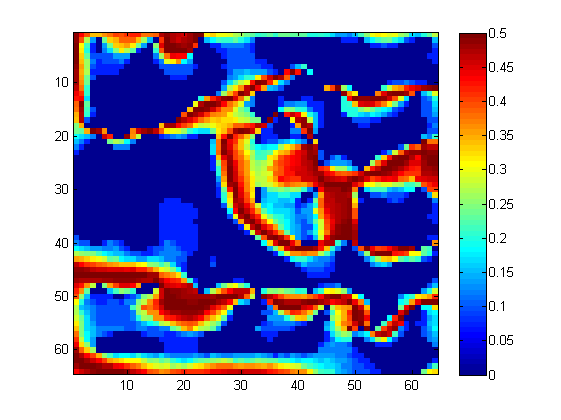
\includegraphics[width=\textwidth]{Figures/SlidesOWP200140903/std_frac_aleat_06_percent_2}
				%\caption{60\% Eq. - 40\% OWP}
			%\end{subfigure}		
			%\begin{subfigure}[b]{0.33\textwidth}
				%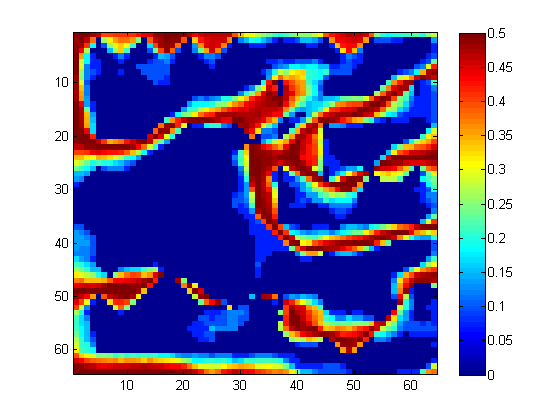
\includegraphics[width=\textwidth]{Figures/SlidesOWP200140903/std_frac_aleat_08_percent_2}
				%\caption{80\% Eq. - 20\% OWP}
			%\end{subfigure}		
			%\begin{subfigure}[b]{0.33\textwidth}
				%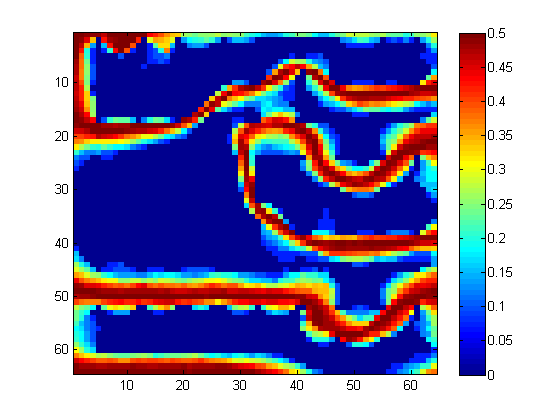
\includegraphics[width=\textwidth]{Figures/SlidesOWP200140903/std_frac_aleat_10_percent_2}
				%\caption{100\% Eq. - 0\% OWP}
			%\end{subfigure}		
%}
%\caption[OWP más muestreo equiespaciado]{\label{fig:owpstd} Imágenes de Desv. Estándar de 200 simulaciones con MPS para distintos porcentajes de muestreo equiespaciado.}
%\end{figure}
%
%
%
%{Experimentos}
%\begin{figure}[H]
%\centering
%\centerline{
			%\begin{subfigure}[b]{0.33\textwidth}
				%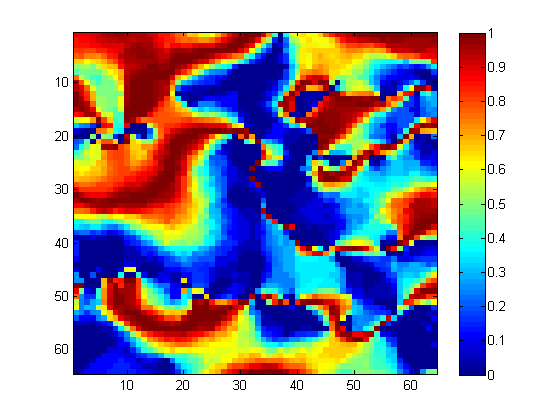
\includegraphics[width=\textwidth]{Figures/SlidesOWP200140903/H_frac_aleat_0_percent_2}
				%\caption{0\% Eq. - 100\% OWP}
			%\end{subfigure}
			%\begin{subfigure}[b]{0.33\textwidth}
				%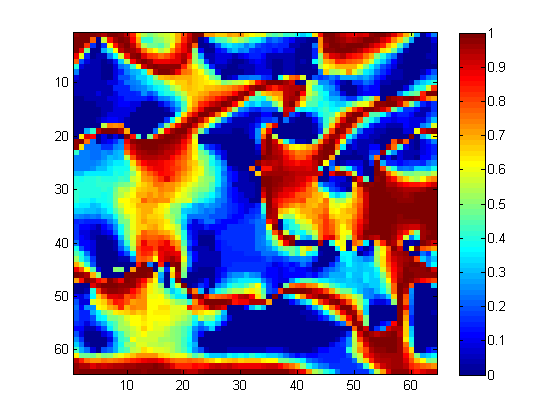
\includegraphics[width=\textwidth]{Figures/SlidesOWP200140903/H_frac_aleat_02_percent_2}
				%\caption{20\% Eq. - 80\% OWP}
			%\end{subfigure}		
			%\begin{subfigure}[b]{0.33\textwidth}
				%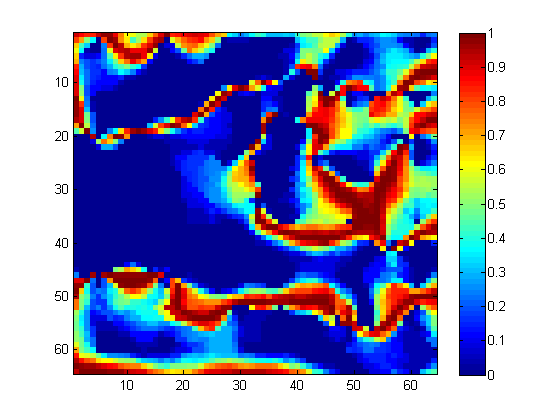
\includegraphics[width=\textwidth]{Figures/SlidesOWP200140903/H_frac_aleat_04_percent_2}
				%\caption{40\% Eq. - 60\% OWP}
			%\end{subfigure}		
%}
%\centerline{
			%\begin{subfigure}[b]{0.33\textwidth}
				%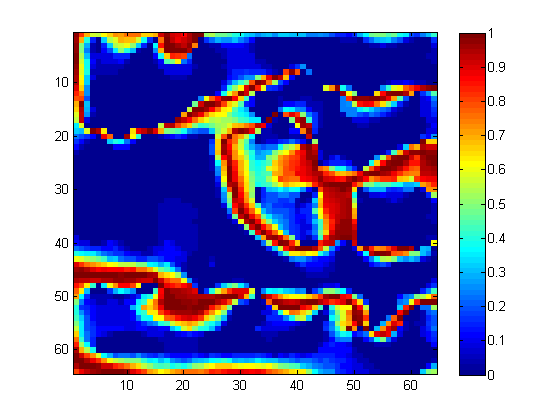
\includegraphics[width=\textwidth]{Figures/SlidesOWP200140903/H_frac_aleat_06_percent_2}
				%\caption{60\% Eq. - 40\% OWP}
			%\end{subfigure}		
			%\begin{subfigure}[b]{0.33\textwidth}
				%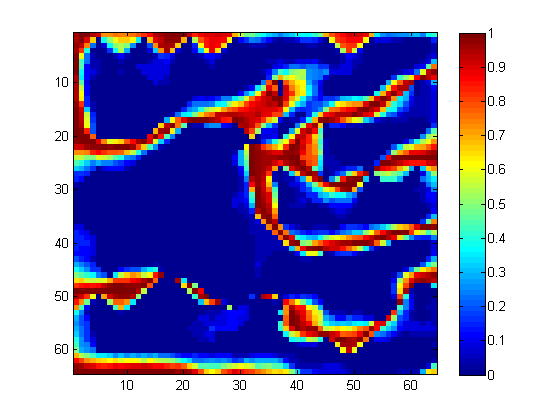
\includegraphics[width=\textwidth]{Figures/SlidesOWP200140903/H_frac_aleat_08_percent_2}
				%\caption{80\% Eq. - 20\% OWP}
			%\end{subfigure}		
			%\begin{subfigure}[b]{0.33\textwidth}
				%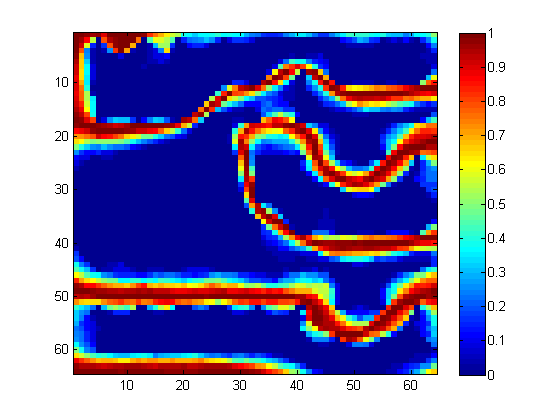
\includegraphics[width=\textwidth]{Figures/SlidesOWP200140903/H_frac_aleat_10_percent_2}
				%\caption{100\% Eq. - 0\% OWP}
			%\end{subfigure}		
%}
%\caption[OWP más muestreo equiespaciado]{\label{fig:owpstd} Imágenes de Entropía de 200 simulaciones con MPS para distintos porcentajes de muestreo equiespaciado.}
%\end{figure}
%
%
%
%{Experimentos}
%{Métricas de calidad de simulaciones}
%La componente $|\mathbf{\sigma}|$ corresponde a la energía total de la imagen de desviación estándar, SNR promedio a el nivel señal a ruido del promedio entre las simulaciones con la imagen original
%\begin{table}
%\centering
  %\begin{center}
  %\resizebox{\columnwidth}{!}{
  %\begin{tabular}{ | c | c | c | c | c | c | c |}
  	%\hline
  	%Métrica & $0\%$ & $20\%$ & $40\%$ & $60\%$ & $80\%$ & $100\%$\\
    %\hline
    %$|\mathbf{\sigma}|$ & 18.2311 & 17.8426 & 13.0801 & 11.1337 & \textbf{10.3974} & 11.605 \\
    %$\text{SNR}$ & 13.9218 & 20.0376 & 23.2711 & \textbf{28.1413}  & 22.9547 & 28.1044 \\
    %\hline   
  %\end{tabular}
  %}
  %\end{center}   
%\end{table}


































%%%%%%%%%%%%%%%%%%%%%%%%%%%%%%%%%%%%%%%%%%%%%%%%%%%%%%%%%%%%%%%%%%%%%%%%%%%%%%%%%%%
%%%%%%%%%%%%%%%%%%%%%%%%%%%%%%%%%%%%%%%%%%%%%%%%%%%%%%%%%%%%%%%%%%%%%%%%%%%%%%%%%%%
%%%%%%%%%%%%%%%%%%%%%%%%%%%%%%%%%%%%%%%%%%%%%%%%%%%%%%%%%%%%%%%%%%%%%%%%%%%%%%%%%%%
%%%%%%%%%%%%%%%%%%%%%%%%%%%%%%%%%%%%%%%%%%%%%%%%%%%%%%%%%%%%%%%%%%%%%%%%%%%%%%%%%%%
%%%%%%%%%%%%%%%%%%%%%%%%%%%%%%%%%%%%%%%%%%%%%%%%%%%%%%%%%%%%%%%%%%%%%%%%%%%%%%%%%%%
%%%%%%%%%%%%%%%%%%%%%%%%%%%%%%%%%%%%%%%%%%%%%%%%%%%%%%%%%%%%%%%%%%%%%%%%%%%%%%%%%%%
%%%%%%%%%%%%%%%%%%%%%%%%%%%%%%%%%%%%%%%%%%%%%%%%%%%%%%%%%%%%%%%%%%%%%%%%%%%%%%%%%%%
%%%%%%%%%%%%%%%%%%%%%%%%%%%%%%%%%%%%%%%%%%%%%%%%%%%%%%%%%%%%%%%%%%%%%%%%%%%%%%%%%%%
%\newpage
%\section{On Noisy Compressive Sensing Formulation}

%\subsection{Size of images and Covariance Matrices}

%As our original Database considered images of size $200$ x $200$, the vectorized signal in canonical and transformed domain (\emph{DCT}) contains $40000$ components and the covariance matrix $C_v$ of the regionalized field requires matrices of size $40000$ x $40000$. Then, the computation of the inverse and square root of $C_v$ required several memory and time to be achieved. In addition, the outcomes of these operations maybe inaccurate at practical precision.

%A basic alternative correspond to reduce the size of the images in the database in order to use more computable covariance matrices. We evaluated the effect of standard resizing methods by the use of the \emph{MATLAB} function \emph{imresize} : \\

			%\begin{itemize}
				%\item $B = imresize(A, scale)$ returns image $B$ that is scale times the size of $A$. The input image $A$ can be a $grayscale$, $RGB$, or $binary imag$e. 
				%\item {By default, \emph{imresize} uses bicubic interpolation.}
				%\item Available Methods
				%\begin{itemize}
					%\item \emph{nearest : } Nearest-neighbor interpolation; the output pixel is assigned the value of the pixel that the point falls within. No other pixels are considered.
					%\item \emph{bilinear: } Bilinear interpolation; the output pixel value is a weighted average of pixels in the nearest 2-by-2 neighborhood.
					%\item \emph{bicubic :} Bicubic interpolation (the default); the output pixel value is a weighted average of pixels in the nearest 4-by-4 neighborhood.
					%\item \emph{box :}	Box-shaped kernel
					%\item{lanczos2 : }	Lanczos-2 kernel
					%\item{lanczos3 : }	Lanczos-3 kernel
				%\end{itemize}
				%\item Parameter and tips
				%\begin{itemize}
					%\item \emph{Antialiasing : }	A Boolean value that specifies whether to perform antialiasing when shrinking an image.
					%\item For bicubic interpolation, the output image may have some values slightly outside the range of pixel values in the input image. This may also occur for user-specified interpolation kernels.
				%\end{itemize}
			%\end{itemize}
%
%
%A second method for resizing image is gaussian pyramidal reduction provided by the function \emph{impyramid} available in \emph{MATLAB} software: \\
%
%\begin{itemize}
				%\item Computes a Gaussian pyramid reduction or expansion of A by one level
				%\item direction can be \emph{reduce} or \emph{expand}
				%\item If A is m-by-n and direction is \emph{reduce}, then the size of B is ceil($\frac{M}{2}$)-by-ceil($\frac{N}{2}$)
				%\item \emph{impyramid} uses the kernel specified on page $533$ of the Burt and Adelson paper \cite{Burt1983,Burt1981}:
				%\begin{itemize}
					%\item 						\[ w = \left[ \frac{1}{4} - \frac{a}{2}, \frac{1}{4} , a , \frac{1}{4} , \frac{1}{4} - \frac{a}{2}   \right]  \]
					%\item {The parameter a is chosen to be $a = 0.375$ so that the equivalent weighting function is close to a Gaussian shape and the weights can be readily applied using fixed-point arithmetic.}
				%\end{itemize}
			%\end{itemize}
%
%
%
%
%
%
%
%
%
%
%








































































































































































